\chapter{Wprowadzenie do dziedziny}
\label{chap:field}

Grafika komputerowa czasu rzeczywistego jest szerokim zagadnieniem.
W tym rozdziale przybliżono podstawowe pojęcia, bibliotekę Vulkan oraz techniki renderowania, których zrozumienie jest wymagane przed rozpoczęciem implementacji silnika graficznego.

\section{Podstawowe pojęcia}
// TODO matematyka
// TODO podział przestrzeni

\section{Vulkan}

Biblioteki graficzne pozwalaja aplikacji na użycie ich API do uzyskania dostępu do akceleracji sprzętowej, czyli przeniesienia obliczeń wymaganych przez renderowanie z CPU do specjalnie pod nie zoptymalizowanego GPU.

Biblioteka graficzna mająca na celu równe wsparcie wielu platform rozwijanych przez różnych IHV (\textit{Independent Hardware Vendor}, niezależny dostawca sprzętu) wymaga drobiazgowego ustandaryzowania i dokumentacji.
W czasie pisania pracy istnieją trzy popularne standardy: Direct3D od firmy Microsoft oraz OpenGL i Vulkan od konsorcjum non-profit Khronos.

Vulkan w wersji 1.0 został po raz pierwszy wydany w 2016. By zacząć używać Vulkan należy pobrać Vulkan SDK rozwijany przez LunarG \cite{VULKANSDK}.
Zawiera on m.in. specyfikację, nagłówki API, biblioteki (de)kompilujące kod SPIR-V oraz warstwy walidacji.

\paragraph{Specyfikacja}

Specyfikacja Vulkan \cite{VULKANSPEC} to ponad 1000 stron zwięzłej, precyzyjnej i szczgółowej specyfikacji API przeznaczonej do użytku zarówno przez implementatorów sterowników, jak i programistów aplikacji. Khronos utrzymuje listę urządzeń, które zaliczyły zestaw testów zgodności Vulkan CTS \cite{VULKANCTS} i spełniają wymagania wieloplatformowości (w odróżnieniu takich API jak DirectX wspieranego tylko przez system Windows i konsole Xbox \cite{HughesDamEtAl13} czy Metal wspierane przeez urządzenia firmy Apple).

\paragraph{Obiektowość i bezstanowość}

Vulkan jest API obiektowym - wszystkie używane koncepty są reprezentowane przez obiekty Vulkan tworzone i niszczone przez aplikację, która ma do nich dostęp poprzez uchwyty.
W przeciwieństwie do OpenGL używającego globalnej maszyny stanów,

Vulkan jest bezstanowy, używany stan jest całkowiecie zaszyty w obiektach i wszystkie funkcje API operują tylko stanie obiektów przekazanych do nich w postaci parametrów i mogą być wywoływane współbieżnie z wielu wątków. Wyjątkiem są parametry zdefiniowane jako \textit{zewnętrznie synchronizowane}, dla których aplikacja musi zagwarantować, że tylko jeden wątek używa obiektu takiego parametu w danym momencie - przykładowo większość funkcji nagrywania poleceń \textit{vkCmd*} wymagają zewnętrznej synchronizacji obiektu bufora poleceń \textit{VkCommandBuffer}, co oznacza, że nagrywanie pojedyńczego bufora poleceń powinno się najlepiej odbywać w ramach jednego wątku.

\paragraph{SPIR-V}

Vulkan używa niskopoziomowej pośredniej reprezentacji shaderów w postaci kodu bajtowego SPIR-V \cite{SPIRVSPEC}, który jest standardem Khronos będącym przenośnym celem kompilacji shaderów napisanych w wysokopoziomowych językach takich jak GLSL, HLSL czy Cg.
Implementatorzy zajmują się tylko translację ze SPIR-V do kodu maszynowego urządzenia, co znacznie upraszcza sterowniki niemuszące osadzać całego kompilatora, przyśpiesza proces kompilacji oraz zmniejsza prawdopodobieństwo sytuacji znanej z OpenGL, w której mimo deklarowanej przenośności API sterowniki różnej jakości interpretują ten sam shader na różne sposoby \cite{GLSLBAD}.

\paragraph{Warstwy}

Vulkan jest niskopioziomowy i skomplikowany w użyciu - słynny tutorial wymaga ponad 1000 linijek kodu C++ do renderowania pojedyńczego trójkąta  \cite{VULKANTUTORIAL}.
Sterowniki nie sprawdzają większości błędów i wymagają od programisty chcącego uniknąć korupcji drobiazgowego przestrzegania zasad poprawnego użycia API.

Na szczęście Vulkan wspiera tworzenie warstw - małych bibliotek dynamicznych pośredniczących pomiędzy apikacją i sterownikiem, które przechwytują wywołania API i pozwala na dodanie do nich dodatkowej logiki.
Vulkan SDK oferuje oficjalne warstwy mające uprościć proces debugowania.

Warstwa walidacji \textit{VK\_LAYER\_KHRONOS\_validation} wykrywaja i raportuje nieprawidłowe i niewydajne użycie API.

Warstwy rozszerzeń implementują funkcje rozszerzeń niewspieranych przez sterownik - przykładowo warstwa \textit{VK\_LAYER\_KHRONOS\_synchronization2} implementuje rozszerzenie \textit{VK\_KHR\_synchronization2}.

Warstwy narzędzi dodają przydatne funkcjonalności takie jak raportowanie wywołań API (\textit{VK\_LAYER\_LUNARG\_api\_dump}), robienie zrzutów ekranu (\textit{VK\_LAYER\_LUNARG\_screenshot}) czy symulacja możliwości bardziej ograniczonych GPU (\textit{VK\_LAYER\_LUNARG\_device\_simulation}).

Warstwy mają negatywny wpływ na wydajność, który jest zwłaszcza widoczny w przypadku warstwy walidacji. Dlatego też warto używać je w trakcie rozwoju, ale nie w produkcie końcowym.

\paragraph{Rozszerzenia}

Nowa funkcjonalność jest dodawana podobnie jak w OpenGL uzywając opcjonalnych rozszerzeń podstawowej specyfikacji. Są one proponowane przez członków Khronos i często są specyficzne dla urządzeń - przykładowo rozszerzenie \textit{VK\_NV\_mesh\_shader} pozwala na użycie shaderów siatki na GPU firmy Nvidia.

Rozszerzenia \textit{EXT} są wspierane przez wielu dostawców. Dostatecznie popularne rozszerzenie może stać się podstawą rozszerzenia \textit{KHR}, od którego oczekuje się wsparcia przez większość sterowników - przykładowo na podstawie rozszerzenia \textit{VK\_NV\_ray\_tracing} stworzono rozszerzenie \textit{VK\_KHR\_ray\_tracing\_pipeline}.

Rozszerzenia mogą być promowana w nowej wersji Vulkan stając się częścią postawowej specyfikacji - przykładowo rozszerzenie \textit{VK\_EXT\_scalar\_block\_layout} zostało promowane w Vulkan 1.2.

\subsection{Podstawy API}

API Vulkan posiadaja regularną i przewidywalną strukturę nazewnictwa oraz użycia obieków.

\subsubsection{Konwencje nazewnictwa}
Konwencje nazewnictwa API Vulkan posiadają regularną i przewidywalną strukturę.
Nagłówek \textit{vulkan.h} dołącza funkcje, struktury, typy wyliczeniowe i stałe preprocesora języka C mające następujące przedrostki:
\begin{itemize}
	\item \textit{vk}: funkcje (np. \textit{vkBeginCommandBuffer}),
	\item \textit{Vk}: struktury i typy wyliczeniowe (np. \textit{VkPipeline} i  \textit{VkPipelineBindPoint}),
	\item \textit{VK\_}: wyliczenia i stałe (np. \textit{VK\_PIPELINE\_BIND\_POINT\_GRAPHICS} i \textit{VK\_NULL\_HANDLE}),
\end{itemize}
W imię zwięzłości dalej w pracy części nazwy będą pomijane jeśli można je wywnioskować z kontekstu - przykładowo \textit{VK\_PIPELINE\_STAGE\_COLOR\_ATTACHMENT\_OUTPUT\_BIT} może być zapisywany jako etap potoku \textit{COLOR\_ATTACHMENT\_OUTPUT}.

Funkcje \textit{vkCmd*()} są nazywane poleceniami i nagrywają polecenie przeznaczone do wykonania na GPU do bufora poleceń - przykładowo polecenie \textit{vkCmdCopyBufferToImage} nagrywa polecenie kopiowania bufora do obrazu.

Funkcje \textit{vkEnumerate*()} i \textit{vkGet*()} służą do odpytywania właściwości obiektów - przykładowo funkcja \textit{vkGetPhysicalDeviceQueueFamilyProperties()} raportuje właściwości rodzin kolejek udostępnianych przez dane urządzenie fizyczne.

Nowe elementy nagłówka wprowadzane przez rozszerzenia kończą się przyrostkami - przykładowo rozszerzenie \textit{VK\_NV\_device\_diagnostic\_checkpoints} wprowadza funkcję \textit{vkCmdSetCheckpointNV} używającą struktury \textit{VkCheckpointDataNV}.

\subsubsection{Model obiektów}

Wszystkie obiekty Vulkan mogą być albo tworzone funkcją \textit{vkCreate*()}, albo alokowane z puli wcześniej utworzonego obiektu funkcją \textit{vkAllocate*()}.

Tworzenie obiektu wymaga przygotowania struktury informacji tworzenia \textit{Vk*CreateInfo}:
\lstset{language=C}
\begin{lstlisting}
Vk*CreateInfo createInfo = {
	.sType = VK_STRUCTURE_TYPE_*_CREATE_INFO;
	.flags = ...,
	...
	.pNext = NULL,
};

Vk* object;
assert(vkCreate*(..., &createInfo, ..., &object) == VK_SUCCESS);
\end{lstlisting}

Alokacja obiektu wymaga przygotowania struktury informacji alokacji \textit{Vk*AllocateInfo}:
\lstset{language=C}
\begin{lstlisting}
Vk*Pool pool;

Vk*AllocateInfo allocInfo = {
	.sType = VK_STRUCTURE_TYPE_*_ALLOCATE_INFO;
	.*Pool = pool,
	...
	.pNext = NULL,
};

Vk* object;
assert(vkAllocate*(..., &allocInfo, ..., &object) == VK_SUCCESS);
\end{lstlisting}

Stworzone obiekty są niszczone funkcją \textit{vkDestroy*()}.
Zaalokowane obiekty są zwalniane funkcją \textit{vkFree*()} lub poprzez zniszczenie puli obiektów.

Struktury Vulkan często wspierają łańcuch \textit{pNext} - wskaźnik \textit{void*} na kolejną strukturę w liście jednokierunkowej lub \textit{NULL}. Jest on używany przez rozszerzenia dodające nowe struktury i może być iterowany w wygodny sposób używając struktur \textit{VkBaseInStructure} i \textit{VkBaseOutStructure} - typ stuktury może być wywnioskowany używając jej pierwszego pola \textit{sType}.

\subsection{Szkielet aplikacji graficznej}

Vulkan, z racji swojej niskopoziomowości, nie narzuca jednej konkretnej struktury aplikacji - większość problemów można rozwiązać wieloma technikami, z których każda ma swoje zalety i wady.
Programista powinien zaprojektować program w taki sposób, żeby rozwiązywał on problem, nie był zawiły i jego profilowanie ujawniało maksymalne użycie GPU.

Wszystkie aplikacjie graficzne mogą być jednak podsumowane następującymi ogólnymi krokami:
\begin{itemize}
	\item Stworzenie bądź wybór podstawowych obiektów: instancja (\textit{VkInstance}), urządzenie fizyczne (\textit{VkPhysicalDevice}), urządzenie logiczne (\textit{VkDevice}) oraz kolejka graficzna (\textit{VkQueue}),
	\item Przygotowanie obiektów służących do prezentacji wyników renderowania: powierzchnia okna (\textit{VkSurface}), łańcuch wymiany (\textit{VkSwapchain}), prezentowalne obrazy (\textit{VkImage}) i ich widoki (\textit{VkImageView}) oraz kolejka prezentacji (\textit{VkQueue}),
	\item Transfer zasobów z CPU do GPU opisanych w zbiorach deskryptorów (\textit{VkDescriptorSet}),
	\item Stworzenie obiektów opisujących proces renderowania: potoki (\textit{VkPipeline}) z shaderami (\textit{VkShaderModule}) oraz przebiegi renderowania (\textit{VkRenderPass}),
	\item Wykonanie procesu renderowania w pętli głównej programu: pobranie nieużywanego prezentowalnego obrazu, nagranie i wykonanie buforów poleceń (\textit{VkCommandBuffer}) realizujących pożądane techniki renderowania oraz prezentacja wyrenderowaniego obrazu.
\end{itemize}

W kolejnych sekcjach pracy przybliżono wspomniane powyżej obiekty Vulkan i zaprezentowano metody ich użycia.


\subsection{Inicjalizacja podstawowych obiektów}

Wszyskie programy używające API Vulkan wymagają wcześniejszego stworzenia obiektów w następującej kolejności:
\begin{itemize}
	\item instancji (\textit{VkInstance}),
	\item powierzchni okna (\textit{VkSurface}),
	\item urządzenia fizycznego (\textit{VkPhysicalDevice}),
	\item urządzenia logicznego (\textit{VkDevice}),
	\item wskaźników funkcji rozszerzeń,
	\item kolejek (VkQueue),
\end{itemize}

Poniższy diagram przedstawia kolejność inicjalizacji podstawowych obiektów Vulkan:
\begin{figure}[H]
	\centering
	\begin{tikzpicture}[node distance=1cm]
		\tikzstyle{object} = [rectangle, minimum width=3cm, minimum height=1cm,text centered, draw=black]
		\tikzstyle{input} = [rectangle, rounded corners, minimum width=3cm, minimum height=5mm,text centered, draw=black]
		\tikzstyle{arrow} = [thick,->,>=stealth]
		\tikzstyle{relation} = [densely dotted,->]
		
		\node (VkInstance) [object] {VkInstance};
		\node (VkApplicationInfo) [input, above = 3mm of VkInstance, rectangle split, rectangle split parts=3] {VkApplicationInfo\nodepart{two}Rozszerzenia instancji\nodepart{three}Warstwy};
		\node (VkSurface) [object, right = of VkInstance] {VkSurface};
		\node (WSI) [input, above = 3mm of VkSurface] {Rozszerzenia WSI};
		\node (VkPhysicalDevice) [object, below = of VkInstance] {VkPhysicalDevice};
		\node (VkDevice) [object, right = of VkPhysicalDevice] {VkDevice};
		\node (VkDeviceInfo) [input, below = 3mm of VkDevice, rectangle split, rectangle split parts=4] {Rodziny kolejek\nodepart{two}Funkcjonalności\nodepart{three}Rozszerzenia urządzenia\nodepart{four}Warstwy};
		\node (VkQueue) [object, right = of VkDevice] {VkQueue};
		
		\draw [arrow] (VkApplicationInfo) -- (VkInstance);
		\draw [arrow] (VkInstance) -- (VkSurface);
		\draw [arrow] (WSI) -- (VkSurface);
		\draw [relation] (VkInstance) -- (VkPhysicalDevice);
		\draw [relation] (VkSurface) -- (VkPhysicalDevice);
		\draw [arrow] (VkPhysicalDevice) -- (VkDevice);
		\draw [arrow] (VkDeviceInfo) -- (VkDevice);
		\draw [relation] (VkDeviceInfo) -- (VkPhysicalDevice);
		\draw [arrow] (VkDevice) -- (VkQueue);
		\draw [relation] (VkDeviceInfo) -- (VkQueue);

		\path ([xshift=29mm,yshift=0mm]current bounding box.south west)
		node[matrix,anchor=south east,cells={nodes={font=\sffamily,anchor=west}},draw,thick,inner sep=1ex]{
			\draw[arrow](0,0) -- ++ (0.6,0); & \node{Tworzenie};\\
			\draw[relation](0,0) -- ++ (0.6,0); & \node{Wybieranie};\\
		};
		
	\end{tikzpicture}
	\caption{Kolejność inicjalizacji podstawowych obiektów Vulkan}
	\label{vulkan_initialization}
\end{figure}

\subsubsection{Instancja}

Pierwszym krokiem każdego programu chcącego używać Vulkan jest stworzenie instancji, która pozwala programowi
na komunikację z loaderem Vulkan.

Loader Vulkan to zewnętrzna warstwa biblioteki Vulkan pośredniczącą miedzy aplikacją i urządzeniami fizycznymi. Jest on odpowiedzialny za wykrywanie sterowników wspierających Vulkan i przekazywanie do nich wywołań API po wcześniejszym przefiltrowaniu ich przez załadowane warstwy.
Poniższy diagram przedstawia warstwową architekturę biblioteki Vulkan \cite{VULKANLOADER}:
\begin{figure}[H]
	\centering
	\begin{tikzpicture}[node distance=1cm]
		\tikzstyle{object} = [rectangle, minimum width=3cm, minimum height=1cm,text centered, draw=black]
		\tikzstyle{relation} = [thick,->,>=stealth]
		
		\node (Aplikacja) [object] {Aplikacja};
		\node (Loader) [object, right = of Aplikacja] {Loader};
		\node (Warstwa1) [object, below = of Aplikacja] {Warstwa \#1};
		\node (WarstwaDot) [right = 2.4mm of Warstwa1] {...};
		\node (WarstwaN) [object, below = of Loader] {Warstwa \#n};
		\node (Driver1) [object, right = of Loader] {Sterownik \#1};
		\node (DriverDot) [below = 3mm of Driver1] {...};
		\node (DriverM) [object, below = 3mm of DriverDot] {Sterownik \#m};
		\node (Device1) [object, right = of Driver1] {Urządzenie fizyczne \#1};
		\node (DeviceDot) [below = 3mm of Device1] {...};
		\node (DeviceK) [object, below = 3mm of DeviceDot] {Urządzenie fizyczne \#k};
		
		\draw [relation] (Aplikacja) -- (Loader);
		\draw [relation] (Loader) -- (Warstwa1);
		\draw [relation] (Warstwa1) -- (WarstwaDot);
		\draw [relation] (WarstwaDot) -- (WarstwaN);
		\draw [relation] (WarstwaN) -- (Loader);
		\draw [relation] (Loader) edge[out=0,in=180] (Driver1);
		\draw [relation] (Loader) edge[out=0,in=180,out looseness=-0.6] (DriverDot);
		\draw [relation] (Loader) edge[out=0,in=180,looseness=0] (DriverM);
		\draw [relation] (Driver1) edge[out=0,in=180] (Device1);
		\draw [relation] (Driver1) edge[out=0,in=180,out looseness=0.2,in looseness=2.4] (DeviceDot);
		\draw [relation] (DriverM) edge[out=0,in=180,looseness=0] (DeviceK);
		\draw [relation] (DriverM) edge[out=0,in=180,out looseness=0.2,in looseness=2.4] (DeviceDot);
		
	\end{tikzpicture}
	\caption{Warstwowa architektura biblioteki Vulkan}
	\label{vulkan_loader}
\end{figure}

Instancja musi zostać stworzona przed użyciem jakichkolwiek innych funkcji API Vulkan.
Jest ona używana przez funkcje instancji, które są używane do:
\begin{itemize}
	\item stworzenia powierzchni okna,
	\item stworzenia komunikatora debugowania,
	\item uzyskania wskaźników funkcji rozszerzeń,
	\item pobrania listy urządzeń fizycznych
\end{itemize}

Podczas tworzenia instancji należy zdefiniować podstawowe informacje o aplikacji (VkApplicationInfo zawierające nazwę i wersję aplikacji, używanego silnika i API Vulkan) oraz listę używanych rozszerzeń instancji i warstw.

\subsubsection{Powierzchnia}

Po stworzeniu instancji Vulkan program chcący prezentować wyniki renderowania musi stworzyć powierzchnię okna.

Ten krok może być pominięty dla programów używających Vulkan w trybie *headless* niewyświetlającym
wyniku renderowania na ekranie. W innym wypadku powierzchnia musi być stworzona przed urządzeniem fizycznym, ponieważ
jest używana do sprawdzania, czy wybrane urządzenie fizyczne będzie wspierało stworzenie łańcucha wymiany dla powierzchni okna.

Stworzenie powierzchni okna odbywa się przy użyciu WSI (Windowing System Integration, integracja systemu okien), który jest zbiórem rozszerzeń udostępnianych przez środowisko uruchomieniowe programu pozwalających na integrację API Vulkan z systemem okien w celu wyświetlenia wyników renderowania.
Użycie WSI wymaga trzech rozszerzeń istancji:
\begin{itemize}
	\item \textit{VK\_KHR\_surface}: udostępnia obiekt VkSurface bez funkcji tworzenia,
	\item \textit{VK\_KHR\_swapchain}: udostępnia obiekt VkSwapchain,
	\item \textit{VK\_KHR\_*\_surface}, gdzie \textit{*} to nazwa systemu okien (przykładowo \textit{VK\_KHR\_win32\_surface} dla Windows): udostępnia specyficzne funkcje instancji pozwalajace na stworzenie VkSurface.
\end{itemize}
Tworzenie okna jest często obsługiwane przez bibliotekę multimedialną taką jak GLFW \cite{GLFW} czy SDL \cite{SDL}, które posiadają funkcjonalność abstrahującą zawiłości tworzenia powierzchni okna używając WSI.

\subsubsection{Urządzenie fizyczne}

Po stworzeniu instancji należy wybrać urządzenie fizyczne. Reprezentuje ono pojedyńczą implementację Vulkan - zwykle jedną z kart graficznych obsługiwana przez zainstalowany sterownik graficzny lub renderer programowy taki jak llvmpipe \cite{LLVMPIPE} czy \cite{SWIFTSHADER}.

Rozróżniane są następujące typy urządzeń fizycznych (\textit{VkPhysicalDeviceType}):
\begin{itemize}
	\item \textit{DISCRETE\_GPU}: dedykowana karta graficzna,
	\item \textit{INTEGRATED\_GPU}: zintegrowane GPU,
	\item \textit{VIRTUAL\_GPU}: wirtualne GPU oferowane przez środowisko wirtualizacji,
	\item \textit{CPU}: renderer programowy.
\end{itemize}

Kazde urządzenie fizyczne jest opisywane ogólnie przy pomocy właściwości i funkcjonalności.
Właściwości (\textit{VkPhysicalDeviceProperties}) zawierają wspieraną wersja API, typ, nazwę i producenta GPU oraz jego limity - numeryczne wartości, które muszą być przestrzegane przez program podczas jego użytkowania (przykładowo limit \textit{maxImageDimension2D} definiuje najwyższa obsługiwana wysokość lub szerokość obrazu 2D).
Funkcjonalności (\textit{VkPhysicalDeviceFeatures} zawierają długą listę wartości logicznych, które opisują dokładnie możliwości urządzenia (przykładowo \textit{tessellationShader} oznaczaja wsparcie shaderów wyliczania teselacji).

Funkcja instancji \textit{vkEnumeratePhysicalDevices()} zwraca listę dostępnych urządzeń fizycznych.
Funkcje \textit{vkGetPhysicalDeviceProperties2()} i \textit{vkGetPhysicalDeviceFeatures2()}\footnote{Te funkcje są częścią rozszerzenia instancji \textit{VK\_KHR\_get\_physical\_device\_properties2}, które zostało promowane w Vulkan 1.1. W przeciwieństwie do wcześniejszych funkcji \textit{vkGetPhysicalDeviceProperties()} i \textit{vkGetPhysicalDeviceFeatures()} używają one fańcucha \textit{pNext} i wspierają odpytywanie właściwości i funkcjonalności wprowadzonych przez późniejsze wesje Vulkan oraz rozszerzenia.} pozwalają on określenie kolejno właściwości i funkcjonalności urządzenia fizycznego.
Funkcja \textit{vkEnumerateDeviceExtensionProperties()} zwraca listę wspieranych rozszerzeń urządzenia.

Aplikacja musi wybrać z listy kandydatów urządzenie fizyczne, które wspiera wszystkie właściwości i funkcjonalności używane podczas działania aplikacji oraz jest najlepiej najwydajniejsze - powinno uniknąć się sytuacji, w której renderer programowy jest wybierany zamiast GPU.


\subsubsection{Urządzenie logiczne}

Po wybraniu urządzenia fizycznego należy użyć go do stworzenia urządzenia logiczne. Reprezentuje ono
sterownik graficzny urządzenia fizycznego i jest używane przez większość funkcji i poleceń Vulkan.

Podczas tworzenia urządzenia fizycznego nalezy zdefiniować używane kolejki oraz funkcjonalności i rozszerzenia urządzenia, których wsparcie było sprawdzane podczs wyboru urządzenia fizycznego.
Dodatkowo w imię kompatybilności wstecznej powinno się ponownie podać listę używanych warstw. Jest to spowodowane przestarzałym i zlikwidowanym podziałem na warstwy instancji i urządzenia - obecnie wszystkie warstwy są traktowane jako oba rodzaje.


\subsubsection{Kolejki}

Podczas tworzenia urządzeniem logicznego sterownik graficzny automatycznie tworzony żądane kolejki.

Kolejki są używane do wykonywania na urządzeniu fizycznym poleceń zawartych w buforach poleceń wysłanych do kolejki funkcją \textit{vkQueueSubmit()}. Funkcja zwraca kontrolę do aplikacji nieczekając na zakończenie wykonywania bufora poleceń na GPU - wymagana jest synchronizacja GPU z CPU przy pomocy ogrodzeń.
Wykonanie buforów poleceń może się odbywać poza kolejnością lub nakładać i wymaga synchronizacji GPU z GPU przy pomocy semafor.
Podobnie nie ma silnej gwarancji porządkowania wykonywania poleceń należącego do pojedyńczego bufora i wymaga jawnej synchronizacji używając barier potoku lub zdarzeń.

Każda kolejka należy do pewnej rodziny kolejek (\textit{VkQueueFlagBits}) sygnalizując tym wsparcie pewnego rodzaju poleceń:
\begin{itemize}
	\item \textit{GRAPHICS}: kolejka graficzna, wspiera polecenia rysowania \textit{vkCmdDraw*()},
	\item \textit{COMPUTE}: kolejka obliczeniowa, wspiera polecenia GPGPU (General-Purpose Computing on GPU, obliczenia ogólnego przeznaczenia na GPU) \textit{vkCmdDispatch*()} oraz polecenia śledzenia promieni (np. \textit{vkCmdTraceRays*()}),
	\item \textit{TRANSFER}: kolejka transferowa, wspiera polecenia transferu (np. \textit{vkCmdCopyBuffer*()}, \textit{vkCmdFillBuffer()}),
	\item \textit{SPARSE\_BINDING}: kolejka zasobów chronionych, wspiera funkcję \textit{vkQueueBindSparse()} dowiązującą do zasobu indywidualne strony pamięci,
	\item \textit{PROTECTED}: kolejka pamięci chronionej, promowana w Vulkan 1.1, pozwala na ochronę pamięci zasobów.
\end{itemize}
Jedna kolejka może należeć do kilku rodzin - przykładowo kolejki graficzne i obliczeniowe zawsze wspierają operacje transferu.
Sterowniki mogą wykonywać bufory poleceń wysłane do różnych kolejek asynchronicznie zapewniając skalowanie na wielordzeniowych GPU, dlatego warto pomyśleć o użyciu osobnych kolejek transferu, graficznych i obliczeniowych do kopiowania danych i przeplatania poleceń rysowania z obliczeniami GPGPU - pamiętając, że narzut związany z synchronizacją może zniwelować poprawy wydajności.

Uchwyt kolejki urządzenia logicznego jest uzyskiwany używając funkcji \textit{vkGetDeviceQueue()}.


\subsubsection{Wskaźniki funkcji rozszerzeń}

Użycie funkcji niebędących częścią używanej wersji API Vulkan i oferowanej przez wspierane rozszerzenia instancji i urządzenia wymaga pobrania wskaźników funkcji w loadera używając funkcji instancji \textit{vkGetInstanceProcAddr()}.
Zwrócony wskaźnik nie musi bezpośrednio wskazywać na implementację oferowaną przez sterownik i może być funkcją loadera wykonującą dodatkową logikę dodaną przez załadowane warstwy.
Funkcja \textit{vkGetDeviceProcAddr()} pozwala na pominięcie loadera, co gwarantuje szybsze wywołania API, ale zwrócona funkcja może być używana tylko dla urządzenia logicznego użytego do pobrania jej.

\subsubsection{Rozszerzenie VK\_EXT\_debug\_utils}

Podczas inicjalizacji Vulkan warto rozważyć użycie rozszerzenia \textit{VK\_EXT\_debug\_utils}, które pozwala na stworzenie komunikatora debugowania (ang. debug messanger) przechwytującego wszystkie komunikaty wygenerowane przez loader, warstwy i sterownik Vulkan.
Przechwycone komunikaty debugowania wraz z priorytetami są przekazywne do wywołania zwrotnego zdefiniowanego przez programistę, które może przykładowo logować wiadomość.
Użycie debuggera wspierającego warunkowe punkty przerwania (ang. conditional breakpoint) dla wiadomości o priorytecie \textit{error} lub \textit{fatal} pozwala na zatrzymanie działania programu tuż po zgłoszeniu błędu przez warstwy walidacji, co upraszcza proces debugownia.

Rozszerzenie pozwala też na dodawanie nazw do obiektów Vulkan funkcją \textit{vkSetDebugUtilsObjectNameEXT()} oraz etykiet do regionów buforów poleceń funkcjami \textit{vkCmdInsertDebugUtilsLabelEXT()}, \textit{vkCmdBeginDebugUtilsLabelEXT()} i \textit{vkCmdEndDebugUtilsLabelEXT()}.

Nazwy i etykiety są używane w wiadomościach debugujących i pokazywane przez zewnętrzne narzędzia takie jak RenderDoc \cite{RENDERDOC}, co znacznie upraszcza proces debugowania.


\subsection{Zasoby}

Vulkan wyróżnia dwa rodzaje zasobów: bufory (\textit{VkBuffer}) i obrazy (\textit{VkImage}).

\subsubsection{Bufory}

Bufor to ciągły blok pamięci który może być odczytany i zapisywany przez GPU. Jest on najprostszym zasobem oferowanym przez Vulkan.
// HIRO bufory


\subsubsection{Obrazy}

Obraz podobnie jak bufor reprezentuje ciągły blok pamięci, ale jego wewnętrzna struktura jest o wiele bardziej skomplikowana i wymaga wcześniejszego ustalenia następujących informacji tworzenia:
\begin{itemize}
	\item typ (\textit{VkImageType})
	\item rozmiar (\textit{VkExtent}),
	\item liczba warstw,
	\item flagi tworzenia (\textit{VkImageCreateFlags}),
	\item liczba poziomów mipmap,
	\item format (\textit{VkFormat}),
	\item liczba próbek na teksel (\textit{VkSampleCountFlagBits}),
	\item kafelkowanie (\textit{VkImageTiling}),
	\item flagi użycia (\textit{VkUsageFlags}),
	\item tryb udostępniania (\textit{VkSharingMode})
	\item początkowy układ (\textit{VkUsageFlags}).
\end{itemize}

// HIRO opisz powyższe

Typ obrazu określa jego liczbę wymiarów (1D, 2D lub 3D).
Rozmiar opisuje liczbę pikseli obrazu (tekseli) wzdłuż każdego wymaiaru (szerokość, wysokość i głębokość).

Obraz Vulkan może być traktowany jako tablica identycznych obrazów, której pojedeńczy element jest zwany warstwą. Warstwy nie są liczone jako wymiar obrazu - obraz 2D z warstwami nie jest obrazem 3D.

Flagi tworzenia pozwalają na definicję dodatkowych funkcjonalności. Przykładowo flaga \textit{CUBE\_COMPATIBLE} pozwala na traktowanie obrazu z 6 kwadratowymi warstwami jako obrazu sześciennego.

Mipmapa to kopia obrazu z każdym wymiarem zmniejszonym dwukrotnie.
W obrazie z mipmapami pierwotny obraz traktuowany jest jako pierwszej mipmapa poziomu zerowego, z której generowane są mipmapy następonych poziomów aż do osiągnięcia wymiaru 1x1x1.
Przykładowo poniższy obraz przedstawia obraz 2D 1024x1024 z modelu Sponza \cite{GLTFSAMPLEMODELS} i jego 10 automatycznie wygenerowanych mipmap:
\begin{figure}[htbp]
	\centering
	\includegraphics[width=0.3\textwidth]{images/mipmap.png}
	\caption{Obraz 2D 1024x1024 z modelu Sponza \cite{GLTFSAMPLEMODELS} i jego 10 mipmap}
	\label{mipmap}
\end{figure}
Obraz posiadający mipmapy zajmuje więcej pamięci, ale pozwala na użycie filtrowania mipmapowego, które jest popularną techniką zwiększającej prędkość i jakość renderowania poprzez wprowadzenie nowych metod filtrowania podczas próbkowania obrazu.

Kafelkowanie obrazu (VkImageTiling) definiuje ułożenie tekselów w pamięci GPU i może być liniowe lub optymalne.
W kafelkowaniu liniowym teksele są uszeregowane w pamięci wierszami (ang. row-major order) podobnie jak tablicach dwuwymiarowych języka C.
Vulkan wspiera też kafelkowanie optymalne, w którym rozkład tekseli obrazu jest decydowany całkowicie przez sterownik - wybrane kafelkowanie ma na celu zwiększenie prędkości dostępu poprzez poprawę lokalności przestrzennej w pamięci podręcznej GPU.

// HIRO próbkowanie, filtrowanie mag, min, mipmap
// HIRO tekstury pozeekranowe

// HIRO pamięć
// HIRO widok
// HIRO bufory uniform i bufory magazynowe, obrazy, próbniki, obrazy magazynowe

\paragraph{Format i przestrzeń kolorów}
Format (\textit{VkFormat}) definiuje rozmiar, strukturę i sposób kodowania podczas zapisu i dekodowania podczas próbkowania pojedyńczego piksela obrazu.
Przestrzeń kolorów (VkColorSpaceKHR) definiuje metodę interpretacji pikseli obrazu przez silnik prezentacji podczas prezentacji obrazu.
Przestrzeń kolorów liniowa (niesprecyzowana) jest używana w obliczeniach shaderów.
Przestrzeń kolorów SRGB jest przeznaczona do wyświetlania na monitorach i jest powszechnia używana w teksturach.
Przykładowe często używane formaty i ich użycie:
\begin{itemize}
	\item \textit{R8G8B8A8\_UNORM}: 4 komponenty koloru B,G,R,A, z których każdy zajmuje 8 bitów i jest interpretowany jako znormalizowana wartość bez znaku (8-bitowa liczba zmienno przecinkowa pomiędzy 0 i 1), używany przez teksturę pozekranowa będącą dołączeniem koloru,
	\item \textit{B8G8R8A8\_SRGB}: podobny do poprzedniego, ale podczas próbkowania GPU przeprowadza automatyczną konwersję z SRGB do przestrzeni liniowej (odwrotna konwersja podczas zapisu), używany przez prezentowalne obrazy łańcucha wymiany,
	\item \textit{D32\_SFLOAT\_S8\_UINT}: 32-bity komponentu głębi (liczba zmiennoprzecinkową ze znakiem), 8-bitów komponentu szablonu (liczba całkowita bez znaku), używany przez bufory głębi.
\end{itemize}


\subsection{Łańcuch wymiany}

Łańcuch wymiany to obiekt \textit{VkSwapchainKHR} będący częścia rozszerzenia \textit{VK\_KHR\_swapchain} WSI i reprezentuje tablica prezentowalnych obrazów należących do powierzchni okna.
Jest on używany do prezentacji obrazu, czyli aktualizacji powierzchni okna zawartością wyrenderowanego obrazu.
Dodatkowo łańcuch wymiany może być używany do synchronizacji pionowej (vertical synchronization, V-sync), czyli synchronizacji prezentacji obrazów z częstotliwością
odświeżania ekranu, której brak powoduje rozrywanie obrazu - korupcję polegającą na jednoczesnym wyświetlaniu zawartości
kilku klatek w tym samym czasie.

Program nie może bezpośrednio prezentować obrazu. Zamiast tego musi on:
\begin{itemize}
	\item Pobrać tablicę uchwytów prezentowalnych obrazów funkcją \textit{vkGetSwapchainImagesKHR()},
	\item Wybrać dostępny prezentowalny obraz z tablicy uchwyrów przy użyciu indeksu zwróconego przez funkcję \textit{vkAcquireNextImageKHR()},
	\item Wyrenderować scenę do dostępnego prezentowalnego obrazu przy użyciu funkcji vkQueueSubmit(),
	\item Oddać wyrenderowany obraz łańcuchowi wymiany funkcją \textit{vkQueuePresentKHR()}.
\end{itemize}
Każdy z tych kroków wymaga synchronizacji z krokiem następnym przy użyciu semaforów. Funkcja \textit{vkAcquireNextImageKHR()} sygnalizuje \textit{semafor dostępności obrazu}, na który czeka funkcja \textit{vkQueueSubmit()} - GPU zaczyna renderowanie dopiero wtedy, gdy prezentowany obraz nie jest używany przez okno.
Funkcja \textit{vkQueueSubmit()} sygnalizuje \textit{semafor zakończena renderowania}, na który czeka funkcja \textit{vkQueuePresentKHR()} - okno może zacząć prezentować wynik renderowania dopiero wtedy, gdy GPU zakończył wykonywanie poleceń.

Prezentacja funkcją \textit{vkQueuePresentKHR()} wymaga użycia uchwytu kolejki prezentacji, która jest dowolną kolejką wspierająca prezentację.
Nie istnieje osobna rodzina kolejek prezentacji, zwykle kolejki graficzne deklarują wsparcie, które może zostać potwierdzone funkcją \textit{vkGetPhysicalDeviceSurfaceSupportKHR()}.

Okno wyświetla tylko jeden prezentowalny obraz na raz, ale istnieje możliwość umieszczania kilku obrazów w kolejce do
prezentacji. Aktualnie prezentowany obraz jest często nazywany \textit{buforem przednim} (front buffer), a reszta obrazów w kolejce od prezentowania jest zwana \textit{buforami tylnymi} (back buffers).

Część sterownika graficznego zwana silnikiem prezentacji wybiera z kolejki obraz służący jako bufor przedni i używa go
do prezentacji. Po zakończeniu prezentacji obraz zostaje oznaczony jako nieużywany i może być ponownie pobrany przez
program.

Poniższy diagram ilustruje cykl życia obrazu łańcucha wymiany:
\begin{figure}[H]
	\centering
	\begin{tikzpicture}[node distance=1cm]
		\tikzstyle{object} = [rectangle, minimum width=3cm, minimum height=1cm,text centered, draw=black]
		\tikzstyle{function} = [rectangle, rounded corners,text centered, draw=black]
		\tikzstyle{arrow} = [thick,->,>=stealth]
		
		\node (PresentableImage1) [object] at (90:4cm) {Prezentowalny obraz};
		\node (PresentableImageDot1) [right = 1mm of PresentableImage1] {...};
		\node (PresentableImages) [draw,dotted,fit=(PresentableImage1) (PresentableImageDot1)] {};
		
		\node (vkAcquireNextImageKHR) [function] at (150:4cm) {vkAcquireNextImageKHR()};
		
		\node (AcquiredImage1) [object] at (180:4cm) {Pobrany obraz};
		\node (AcquiredImageDot1) [left = 1mm of AcquiredImage1] {...};	
		\node (AcquiredImages) [draw,dotted,fit=(AcquiredImage1) (AcquiredImageDot1)] {};
		
		\node (vkQueueSubmit) [function] at (215:4cm) {vkQueueSubmit()};
		
		\node (RenderedImage1) [object] at (270:4cm) {Wyrenderowany obraz};
		\node (RenderedImageDot1) [right = 1mm of RenderedImage1] {...};	
		\node (RenderedImages) [draw,dotted,fit=(RenderedImage1) (RenderedImageDot1)] {};
		
		\node (vkQueuePresentKHR) [function] at (325:4cm) {vkQueuePresentKHR()};
		
		\node (PresentedImage1) [object] at (360:4cm) {Prezentowany obraz};
		\node (PresentedImageDot1) [right = 1mm of PresentedImage1] {...};	
		\node (PresentedImages) [draw,dotted,fit=(PresentedImage1) (PresentedImageDot1)] {};
		
		\node (PresentEvent) [function] at (390:4cm) {Wyświetlenie obrazu};
				
		\draw [arrow] (120:4cm) arc (120:142:4cm);
		\draw [arrow] (157:4cm) arc (157:168:4cm);
		\draw [arrow] (198:4cm) arc (198:208:4cm);
		\draw [arrow] (224:4cm) arc (224:240:4cm);
		\draw [arrow] (307:4cm) arc (307:318:4cm);
		\draw [arrow] (335:4cm) arc (335:343:4cm);
		\draw [arrow] (372:4cm) arc (372:383:4cm);
		\draw [arrow] (399:4cm) arc (398:412:4cm);
		
		\node (PresentableImagesLabel)[above=0cm of PresentableImages] {\textbf{Nieużywane prezentowalne obrazy}};
		\node (AcquiredImagesLabel)[below=0cm of AcquiredImages] {\textbf{Pobrane obrazy}};
		\node (RenderedImagesLabel)[below=0cm of RenderedImages] {\textbf{Wyniki renderowania}};
		\node (PresentedImagesLabel)[below=0cm of PresentedImages] {\textbf{Kolejka obrazów do prezentacji}};
		
		\draw [arrow, postaction={decorate,decoration={text along path,raise=1mm,text align=center,text={Aplikacja}}}] (133:16mm) arc (133:300:16mm);
		\draw [arrow, postaction={decorate,decoration={text along path,raise=1mm,text align=center,reverse path,text={Łańcuch wymiany}}}] (305:16mm) arc (305:486:16mm);
		
		
	\end{tikzpicture}
	\caption{Cykl życia obrazu łańcucha wymiany}
	\label{swap_chain}
\end{figure}

Informacje tworzenia łańcucha wymiany muszą być wspierane przez powierzchnię okna.
Wymaganie jest ustalenei trybu prezentacji (funkcja \textit{vkGetPhysicalDeviceSurfacePresentModesKHR()}), liczba prezentowalnych obrazów i ich rozmiar (funkcja \textit{vkGetPhysicalDeviceSurfaceFormatsKHR()}) oraz ich formatu i przestrzeń kolorów (funkcja \textit{vkGetPhysicalDeviceSurfaceCapabilitiesKHR()}).

Trybu prezentacji (\textit{VkPresentModeKHR}) definiuje dokładny mechanizm działania silnika prezentacji:
\begin{itemize}
	\item \textit{IMMEDIATE}: wyrenderowane obrazy są natychmiastowo prezentowane. Brak synchronizacji pionowej może powodować rozrywanie obrazu.
	\item \textit{FIFO}: łańcuch wymiany zachowuje się jak kolejka FIFO. Przed odświeżeniem ekranu obraz z przodu kolejki jest usuwany i prezentowany. Wyrenderowane obrazy są dodawane na koniec kolejki. Jeśli kolejka jest pełna, to program jest blokowany na funkcji \textit{vkQueuePresentKHR()} i musi czekać na zwolnienie miejsca w kolejce. Ten tryb zapewnia synchronizację pionową i jego dostępność jest gwarantowana przez specyfikację Vulkan. Jednak w sytuacji, w której GPU renderuje obrazy szybciej, niż ekran je prezentuje, program jest blokowany.
	\item \textit{FIFO\_RELAXED}: podobny do \textit{FIFO}, ale prezentacja obrazu może pomijać synchronizację pionowa wywołując rozrywanie gdy kolejka jest pełna, ale zmniejszając czas blokowania aplikacji,
	\item \textit{MAILBOX}: podobny do \textit{FIFO}, ale zamiast blokowania programu gdy kolejka jest pełna, starsze obrazy w kolejce są zastępowane przez nowsze. Ten tryb zapewnia synchronizację pionową i zgodnie ze specyfiakcją Vulkan gwarantuje, że program nie jest blokowany podczas prezentacji oraz może zawsze pobrać nieużywany obraz z łańcucha wymiany, ale tylko pod warunkiem, że liczba prezentowalnych obrazów jest większa od minimalnej liczby wymaganej przez powierzchnię okna.
\end{itemize}

Po stworzeniu łańcucha obrazów aplikacja może pobrać tablicę uchwytów jego prezentowalnych obrazów funkcją \textit{vkGetSwapchainImagesKHR()} - należy oczywiście pamiętać, że pomimo posiadania uchwytu obrazu może być on używany dopiero, gdy jego indeks jest zwrócony przez funkcję \textit{vkAcquireNextImageKHR()}.
Następnie należy utworzyć widoki prezentowalnych obrazów, które będą później używane do renderowania do nich.

Istnieją sytuacja, w których łańcuch wymiany musi być odtworzony (zniszczony i stworzony).
Fukcje \textit{vkAcquireNextImageKHR()} i \textit{vkQueuePresentKHR()} mogą zwrócić rezultat
ERROR\_OUT\_OF\_DATE\_KHR oznaczający, że powierzchnia okna zmieniła się w taki sposób, że nie jest już kompatybilna z łańcuchem wymiany.
Aplikacja może chciać odtworzyć łańcuch wymiany także dla rezultatu \textit{SUBOPTIMAL\_KHR} oznaczającego, że rozmiar obrazów łańcucha wymiany przestał dokładnie pokrywać się z powierzchnią okna i prezentacja musi przeprowadzać dodatkowe operacje skalowania.
Najczęstszym sprawcą obu tych sytuacji jest zmiana rozmiaru okna.


\subsection{Bufory poleceń}

// TODO diagram stanu,

// TODO Rodzaje poleceń: zmiana stanu (dowiązywanie), rysowanie

// TODO ponowne użycie vs nagrywanie co klatkę

\subsection{Synchronizacja}

// TODO wstęp o synchronizacji

\subsubsection{Bariery potoku}

Bariera potoku to prymityw synchronizacji definiowany poleceniem \textit{vkCmdPipelineBarrier()} pozwalający na zdefiniowanie zależności wykonania oraz zależności pamięci pomiędzy poleceniami przed i po barierze.

Zależność wykonania to gwarancja, że praca pewnych \textit{źródłowych etapów potoku} (określonych używając
\textit{VkPipelineStageFlags}) dla wcześniejszego zestawu poleceń została zakończona przed rozpoczęciem wykonywania pewnych
\textit{docelowych etapów potoku} dla późniejszego etapu poleceń. 

Przykładowo zależność wykonania pomiędzy etapami
\textit{COLOR\_ATTACHMENT\_OUTPUT} i \textit{FRAGMENT\_SHADER} gwarantuje, że zapis do dołączeń kolorów został skończony przed rozpoczęciem
wykonywania shadera fragmentów.

Zależność pamięci to zależność wykonania z dodatkową gwarancją, że rezultat zapisów wyspecyfikowanych przez pewien \textit{źródłowy
zakres dostępów} (określony używając \textit{VkAccessFlags}) wygenerowanych przez wcześniejszy zestaw poleceń jest udostępiony
późniejszemu zestawowi poleceń dla pewnego \textit{docelowego zakresu dostępów}.

Przykładowo zaleźność pamięci pomiędzy etapami
\textit{COLOR\_ATTACHMENT\_OUTPUT} i \textit{FRAGMENT\_SHADER} z zakresami dostępów \textit{COLOR\_ATTACHMENT\_WRITE} i \textit{SHADER\_READ} gwarantuje, że zapis
do dołączeń kolorów zostanie skończony i będzie mógł być odczytany przez shader fragmentów.

Istnieją trzy rodzaje barier w zależności od rodzaju pamięci zarządzanego przez zależności pamięci:

\begin{itemize}
	\item {bariery pamięci obrazów}: dla zakresu obrazu, dodatkowo pozwala na tranzycje układu obrazu,
	\item {bariery pamięci buforów}: dla zakresu bufora,
	\item {globalne bariery pamięci}: dla wszystkich istniejących obiektów,
\end{itemize}

// TODO użycie
// TODO listingi?

\subsubsection{Semafory}

Semafory to obiekty \textit{VkSemaphore} pozwalające na synchronizację wykonywania buforów poleceń w tej samej lub pomiędzy kolejkami. GPU
może sygnalizować semafor po zakończeniu wykonywania poleceń oraz może czekać na sygnalizację semafora przed
rozpoczęciem wykonywania następnego bufora poleceń.

Przykładowo semafory są używane do synchronizacji pomiędzy kolejką
graficzna i kolejką prezentacji w celu zagwarantowania, że prezentowalny obraz łańcucha wymiany jest używany tylko przez jedną kolejkę.

\subsubsection{Ogrodzenia}

Ogrodzenia to obiekty \textit{VkFence} pozwalające na synchonizację poleceń wykonywanych w kolejce na GPU z CPU.
Ogrodzenie może być sygnalizowane przez GPU po zakończeniu wykonywania funkcji używających GPU, CPU może zresetować ogrodzenie
funkcją \textit{vkResetFences()} lub czekać na jego sygnalizację funkcją \textit{vkWaitForFences()} chwilowo blokując wykonywanie programu.

Przykładowo ogrodzenia są używane do zagwarantowania, że program nie używa funkcji \textit{vkQueueSubmit()} do wysyłania buforów poleceń szybciej, niż GPU je wykonuje.

\subsubsection{Zdarzenia}
Zdarzenia to obiekty \textit{VkEvent} pozwalające ogólną synchronizację wykonywanych poleceń z innymi poleceniami bądź CPU.
Funkcja \textit{vkCmdSetEvents()} sygnalizuje zdarzenie po rozpoczęciu wykonywania źródłowych etapów potoku zależności wykonania. Wraz z funkcją \textit{vkCmdWaitEvents()} pozwala na specyfikację pełnej zależności pamięci.
Aplikacja może manualnie sygnalizowane, resetować i czekać na zdarzenia na funkcjami \textit{vkSetEvents()}, \textit{vkResetEvent()} i \textit{vkGetEventStatus()}, co pozwala na blokowanie GPU przez CPU i jest jedyną funkcjonalnością niemożliwą do zaimplementowania przez poprzednio opisane prymitywy synchronizacji, które powinny być optymalniejsze od elastyczniejszych zdarzeń.

\subsection{Deskryptory i stałe push}

Vulkan nie pozwala na bezpośredni dostęp do zasobów z poziomu shadera i wymaga użycia deskryptorów.

Deskryptor to blok pamięci z opisem pojedyńczego zasobu używanego przez GPU. Dokładna wewnętrzna struktura deskryptora jest w formacie specyficznym dla GPU \cite{DESCRIPTORSHARD}, ale może być intuicyjnie rozumiana jako struktura zawierająca wskaźnik to adresu pamięci GPU z danymi zasobu oraz dodatkowe metadane opisujące rodzaj zasobu oraz w jaki sposób zasób będzie używany przez shader.

\subsubsection{Tworzenie deskryptorów}

Vulkan nie pozwala na tworzenie i używanie pojedyńczych deskryptorów i wymaga grupowania ich w tablice poprzez zbiory deskryptorów  (obiekt \textit{VkDescriptorSet}).

Stworzenie zbiorów deskryptorów wymaga wcześniejszego stworzenia dwóch obiektów: puli deskryptorów (\textit{VkDescriptorPool})
oraz układu zbioru deskryptorów (\textit{VkDescriptorSetLayout}).

Pula deskryptorów to źródło, z którego alokowane są deskryptory w postaci zbiorów deskryptorów. Podczas tworzenia należy zadeklarować:
\begin{itemize}
	\item maksymalną liczbę zaalokowanych zbiorów deskryptorów,
	\item maksymalną liczbę rodzajów deskryptorów.
\end{itemize}

Układ zbioru deskryptorów reprezentuje wewnętrzną strukturę zbioru deskryptorów - programista języka C może o nim myśleć jako o deklaracji struktury używanej później do definiowania zmiennych (zbiorów deskryptorów).
Układ składa się z listy dowiązań deskryptorów (\textit{VkDescriptorSetLayoutBinding}).

Jedno dowiązanie deskryptora reprezentuje fragment zbioru deskryptorów zajmowany przez deskryptory tego samego typu.
Każde dowiązanie deskryptora jest opisane poprzez:
\begin{itemize}
	\item {\textit{numer dowiązania}}: używany do odnoszenia się w shaderze do dowiązania i uzyskania dostępu do
	zasobu,
	\item \textit{typ deskryptora},
	\item \textit{liczba deskryptorów},
	\item {\textit{zbiór etapów cieniowania}}: określa które shadery w potoku graficznym mają dostep do zasobów.
\end{itemize}
Typ deskryptora zależy od rodzaju opisywanego zasobu, przykładowo:
\begin{itemize}
	\item {\textit{UNIFORM\_BUFFER}}: bufor uniform,
	\item {\textit{UNIFORM\_BUFFER\_DYNAMIC}}: dynamiczny bufor uniform, dodatkowy dynamiczny offset jest specyfikowany podczas dowiązywania zbioru deskryptorów,
	\item {\textit{STORAGE\_BUFFER}}: bufor magazynowy,
	\item {\textit{STORAGE\_BUFFER\_DYNAMIC}}: dynamiczny bufor magazynowy,
	\item {\textit{SAMPLER}}: próbnik,
	\item {\textit{SAMPLED\_IMAGE}}: widok próbkowalnego obrazu,
	\item {\textit{STORAGE\_IMAGE}}: widok obrazu magazynowego,
	\item {\textit{COMBINED\_IMAGE\_SAMPLER}}: próbkowany obraz, pojedyńczy deskryptor jest skojarzony zarówno z próbnikiej, jaki i z widokiem obrazu,
	\item {\textit{UNIFORM\_TEXEL\_BUFFER}}: widok bufora uniform,
	\item {\textit{STORAGE\_TEXEL\_BUFFER}}: widok bufora magazynowego.
\end{itemize}

\subsubsection{Aktualizacja deskryptorów}

Po stworzeniu zbioru deskryptorów zawartość jego deskryptorów jest niezdefiniowna i musi być zaktualizowana funkcją
\textit{vkUpdateDescriptorSets()}. Jej wejściem jest \textit{tablica struktur VkWriteDescriptorSet}, której każdy pojedyńczy element opisuje
który wycinek tablicy wybranego dowiązania w zbiorze deskryptorów powinien być zaktualizowany informacjami o zasobach.

Aktualizacja zbioru deskryptorów odbywa się na CPU natychmiastowo po wywołaniu \textit{vkUpdateDescriptorSets()} i jest możliwa
tylko zanim zbiór deskryptorów zostanie użyty przez jakiekolwiek polecenie w nagrywanym bądź wykonywanym buforze poleceń.
Jednym z wyjątków jest aktualizacja zbiorów deskryptorów zaalokowanych z puli deskryptorów wspierającej funkcjonalność uaktualnienia deskryptorów po dowiązaniu.

\subsubsection{Stałe push}

Stałe push to sposób przekazywania danych do shaderów będący szybszą i łatwiejszą 
alternatywą dla deskryptorów. Nie wymagają one tworzenia i aktualizacji zasobów opartych na pamięci GPU - pamięć CPU stałej push jest bezpośrednio kopiowana i przechowywana w nagrywanym buforze poleceń komendą \textit{vkCmdPushConstants()}.

Niestety ta metoda ma poważne ograniczenie - minimalny rozmiar pamięci udostępniany shaderowi gwarantowany przez specyfikację Vulkan to tylko 128 bajtów, co odpowiada dwóm macierzom 4x4. Z tego powodu stałe push powinny być używane do przekazywania danych, które zmieniają się na tyle często, że narzut wydajnościowy synchronizacji modyfikowanych buforów uniform. Przykładem mogą być macierze transformacji albo indeksy tekstur używane przez polecenia rysowania.


\subsubsection{Zadeklarowanie użycia deskryptorów w układzie potoku}

Układ potoku (\textit{VkPipelineLayout}) zawiera informacje o sposobie organizacji wszystkich zbiorów deskryptorów i stałych push, które mogą być używane w potoku (\textit{VkPipeline}). Jest on używany do dowiązywania zbiorów deskryptorów i nagrywania stałych push.

Podczas tworzenia należy zadeklarować:
\begin{itemize}
	\item listę układów zbiorów deskryptorów,
	\item listę zakresów stałych push (\textit{VkPushConstantRange}).
\end{itemize}

Zakres stałej push składa się z:
\begin{itemize}
	\item zbioru etapów cieniowania mających dostęp do stałej push,
	\item offset i rozmiar pamięci, który moze być używany przez powyższe etapy cieniowania.
\end{itemize}

Liczba poszczególnych typów deskryptorów uzwględnionych w potoku renderowania jest ograniczona limitami urządzenia fizycznego.
Limit \textit{maxPerStageResources} to maksymalna liczba zasobów, które mogą być dostępne dla pojedyńczego etapu cieniowania.
Rodzina limitów \textit{maxDescriptorSet*}, gdzie \textit{*} to typ deskryptora, kontroluje maksymalną liczbę deskryptorów danego typu w układzie potoku.

\subsubsection{Dowiązanie deskryptorów do bufora poleceń}

Przed użyciem zasobów opisanych zbiorem deskryptorów przez polecenia rysowania wymagane jest dowiązania ich do bufora
poleceń przy użyciu komeny \textit{vkCmdBindDescriptorSets()}. Jednym z jej wejść jest \textit{numer zbioru}, który wraz z numerami
dowiązań służy do identyfikacji zasobu w shaderach.


\subsubsection{Diagram użycia deskryptorów}

Relacje pomiędzy obiektami, funkcjami i komendami używającymi deskryptorów i stałych push zostały przedstawione na poniższym diagramie:
\begin{figure}[H]
	\centering
	\begin{tikzpicture}[node distance=1cm]
		\tikzstyle{object} = [rectangle, minimum width=3cm, minimum height=1cm,text centered, draw=black]
		\tikzstyle{function} = [rectangle, rounded corners,text centered, draw=black]
		\tikzstyle{arrow} = [thick,->,>=stealth]
		\tikzstyle{relation} = [densely dotted]

		\node (VkDescriptorSetLayout) [object] {VkDescriptorSetLayout};
		\node (VkDescriptorPool) [object, right = of VkDescriptorSetLayout] {VkDescriptorPool};
		\node (VkDescriptorSet) [object, below = of VkDescriptorPool] {VkDescriptorSet};
		\draw [arrow] (VkDescriptorSetLayout) -- (VkDescriptorSet);
		\draw [arrow] (VkDescriptorPool) -- (VkDescriptorSet);
		
		\node (VkPipelineLayout) [object, below = of VkDescriptorSetLayout] {VkPipelineLayout};
		\node (VkPushConstantRange) [object, left = of VkDescriptorSetLayout] {VkPushConstantRange};
		\draw [arrow] (VkDescriptorSetLayout) -- (VkPipelineLayout);
		\draw [arrow] (VkPushConstantRange) -- (VkPipelineLayout);
		
		\node (vkUpdateDescriptorSets) [function, right = of VkDescriptorSet] {vkUpdateDescriptorSets};
		\draw [arrow] (VkDescriptorSet) -- (vkUpdateDescriptorSets);
		\draw [arrow] (vkUpdateDescriptorSets) -- (VkDescriptorSet);
		\node (resources) [object, rectangle split, rectangle split parts=2, above = of vkUpdateDescriptorSets] {VkBuffer \nodepart{two} VkImage};
		\draw [arrow] (resources) -- (vkUpdateDescriptorSets);
		\draw [relation] (resources) edge[out=135, in=45, looseness=0.4] (VkDescriptorSetLayout);
		
		\node (vkCmdBindDescriptorSets) [function, below = of VkDescriptorSet] {vkCmdBindDescriptorSets};
		\draw [arrow] (VkPipelineLayout) -- (vkCmdBindDescriptorSets);
		\draw [arrow] (VkDescriptorSet) -- (vkCmdBindDescriptorSets);
		
		\node (vkCmdPushConstants) [function, below = of VkPipelineLayout] {vkCmdPushConstants};
		\draw [arrow] (VkPipelineLayout) -- (vkCmdPushConstants);
		\node (pushmemory) [object, text width=2cm, left = of vkCmdPushConstants] {pamięć CPU stałej push};
		\draw [arrow] (pushmemory) -- (vkCmdPushConstants);
		\draw [relation] (pushmemory) -- (VkPushConstantRange);
		
		\node (VkCommandBuffer) [object, below = of vkCmdBindDescriptorSets] {VkCommandBuffer};
		\draw [arrow] (vkCmdPushConstants) -- (VkCommandBuffer);
		\draw [arrow] (vkCmdBindDescriptorSets) -- (VkCommandBuffer);
		
		 \path ([xshift=34mm,yshift=-2mm]current bounding box.south west)
		node[matrix,anchor=south east,cells={nodes={font=\sffamily,anchor=west}},
		draw,thick,inner sep=1ex]{
			\draw[arrow](0,0) -- ++ (0.6,0); & \node{Użycie};\\
			\draw[relation](0,0) -- ++ (0.6,0); & \node{Kompatybilność};\\
		};

	\end{tikzpicture}
	\caption{Relacje pomiędzy obiektami Vulkan używanymi do zarządzania deskryptorami}
	\label{descriptor_relations}
\end{figure}

\subsubsection{Dostęp do zasobów w shaderach}

Po dowiązaniu zbiorów deskryptorów i stałych push do bufora poleceń dostęp do zasobów z poziomu kodzu GLSL shadera odbywa się poprzez zmienną posiadającą odpowiednie kwalifikatory układu.

Przykładowo kwalifikator układu dla pojedyńczego deskryptora typu UNIFORM\_BUFFER z dowiązania o numerze $x$ ze zbioru o numerze $y$ ma następującą formę:
\lstset{language=GLSL}
\begin{lstlisting}
struct bufferStruct {
	vec3 field1;
	mat4 field2;
	...
};
layout(scalar, set = y, binding = x) uniform bufferBlock {
	bufferStruct buffer;
};
\end{lstlisting}

Analogicznie kwalifikator układu dla tablicy deskryptorów typu COMBINED\_IMAGE\_SAMPLER o rozmiarze $r$ z dowiązania o numerze $x$ ze zbioru o numerze $y$ próbkowanych obrazów 2D ma następującą formę:
\lstset{language=GLSL}
\begin{lstlisting}
layout(set = y, binding = x) uniform sampler2D texture[r];
\end{lstlisting}


\subsubsection{Układ pamięci scalar dla buforów i stałych push}

Układ pamięci definiuje wyrównania pól w strukturze znajdującej się w opisywanym deskryptorem pamięci.
Używany układ musi być zadeklarowany w kwalifikatorze układu dla buforów i stałych push.

OpenGL wspiera dwa rodzaje standardy układów: \textit{std140} i \textit{std430}.
Vulkan odziedziczył te układy i dodatkowo wprowadził \textit{scalar}.
Każdy kolejny standard pozwala na ciaśniejsze upakowanie pól, co skutkuje mniejszym zużyciem pamięci GPU.

Układ pamięci scalar wymaga ona wsparcia funkcjonalności urządzenia Vulkan 1.2 \textit{scalarBlockLayout}, które w czasie pisania pracy jest wspierane przez więcej niż $98\%$ urządzeń \cite{GPUINFO}.
Dodatkowo kod GLSL shadera musi posiadać następującą dyrektywę preprocesora:
\lstset{language=GLSL}
\begin{lstlisting}
#extension GL_EXT_scalar_block_layout : require
\end{lstlisting}

W przeciwieństwie do swoich poprzedników, układ scalar ma bardzo proste wymagania dotyczące wyrównań pól:
\begin{itemize}
	\item dla typu skalarnego jest równe jego wielkości,
	\item dla wektora bądź macierzy jest równe wyrównaniu jego komponentu,
	\item dla tablicy jest równe wyrównaniu jego elementu,
	\item dla struktury jest równe największemu wyrównaniu jej pól.
\end{itemize}
Powyższe zasady skutkują maksymalnym upakowaniem pól dla buforów używających tylko standardowych 32-bitowych skalarów mających to samo wyrównanie, co obejmuje większość shaderów nieużywających rozszerzeń takich jak \textit{GL\_EXT\_shader\_16bit\_storage} wprowadzające 16-bitowe skalary.


\section{Rozszerzenie VK\_EXT\_descriptor\_indexing}

Rozszerzenie \textit{VK\_EXT\_descriptor\_indexing} wprowadziło szereg dodatkowych funkcjonalności pozwalających na tworzenie dużych zbiorów
deskryptorów zawierających wszystkie zasoby używane przez program.
Celem tego jest umożliwienie technik renderowania bez dowiązań. Z powodu swojej użyteczności rozszerzenie to zostało promowane w Vulkan 1.2.
W kolejnych sekcjach opisano nowe funkcjonalości.

\subsection{Niejednolite dynamiczne indeksowanie deskryptorów}

Deskryptory są traktowane przez shadery jako tablice, do których dostęp odbywa się używając indeksu.

Statyczne indeksowanie pozwala na dostęp do zasobu przy użyciu indeksu będącego stałą czasu kompilacji. Jest to najstarszy i zawsze wspierany sposób indeksowania.

Dynamiczne indeksowanie pozwala na dostęp do zasobu przy użyciu wartości czasu wykonywania.

Jednolite dynamiczne indeksowanie wymaga, żeby indeks był taki sam we wszystkich wywołań shadera spowodowanych przez pojedyńcze polecenie rysowania - użycie różnych indeksów jest błędem i może skutkować korupcjami.
Przykładem tego rodzaju indeksowania jest użycie indeksu tekstury w stałej push lub buforze uniform.
Wymaga ona wsparcia następujących funkcjonalności urządzenia Vulkan 1.0:
\begin{itemize}
	\item {\textit{shaderUniformBufferArrayDynamicIndexing}}: tablice buforów uniform,
	\item {\textit{shaderSampledImageArrayDynamicIndexing}}: tablice próbkowalnych obrazów,
	\item {\textit{shaderStorageBufferArrayDynamicIndexing}}: tablice buforów magazynowych,
	\item {\textit{shaderStorageImageArrayDynamicIndexing}}: tablice obrazów magazynowych.
\end{itemize}

Niejednolite dynamiczne indeksowanie pozwala na swobodny dostęp do zasobów znajdujących się w pamięci GPU przy użyciu dowolnych indeksów.
Przykładem może być indeksowanie tablicy tekstur używając indeksu instancji polecenia rysowania albo próbki tekstury pozaekranowej.
Wymaga ona wsparcia analogicznych funkcjonalności urządzenia Vulkan 1.2:
\begin{itemize}
	\item {\textit{shaderUniformBufferArrayNonUniformIndexing}},
	\item {\textit{shaderSampledImageArrayNonUniformIndexing}},
	\item {\textit{shaderStorageBufferArrayNonUniformIndexing}},
	\item {\textit{shaderStorageImageArrayNonUniformIndexing}}.
\end{itemize}

W czasie pisania pracy powyższe funkcjonalności są wspierane przez więcej niż $90\%$ urządzeń \cite{GPUINFO}.

Niejednolite dynamiczne indeksowanie wymaga zadeklarowania rozszerzenia SPIR-V \textit{SPV\_EXT\_descriptor\_indexing}.
Może być to uczynione z poziomu kodu GLSL przez dodanie następującej dyrektywy preprocesora:
\lstset{language=GLSL}
\begin{lstlisting}
#extension GL_EXT_nonuniform_qualifier : require
\end{lstlisting}
Dodatkowo każde użycie niejednolitego indeksu powinno być oznaczone funkcją \textit{nonuniformEXT}:
\lstset{language=GLSL}
\begin{lstlisting}
vec4 color = texture(textures2D[nonuniformEXT(index)], uv);
\end{lstlisting}

Wymóg jednolitości podczas indeksowania deskryptorów był spowodowany ograniczeniami poprzednich generacji GPU - w modelu renderowania OpenGL dostęp do dowiązanych tekstur odbywał się pośrednio poprzez jednostki teksturujące, które były widoczne przez wszystkie wywołania shaderów i nie pozwalały na zmianę dołączonych tekstur podczas wykonywania polecenia rysowania \cite{GPUGEM4}. 

\subsection {Aktualizacja deskryptorów po dowiązaniu}

Domyślnie deskryptory nie mogą być aktualizowane po nagraniu ich dowiązania w buforze poleceń, przez co aplikacja musi mieć kompletną wiedzę o wszystkich używanych zasobach w trakcie nagrywania buforów poleceń.
Nie dotyczy to jednak deskryptorów używających funkcjonalności aktualizacji po dowiązaniu, co pozwala na elastyczniejsze zarządzanie zasobami poprzez odroczenie aktualizacji zbiorów deskryptorów aż do momentu bezpośrednio przed wykonaniem bufora poleceń.

Wsparcie aktualizacji po dowiązaniu dla wybranego typu deskryptora wymaga odpowiedniej funkcjonalności urządzenia Vulkan 1.2:
\begin{itemize}
	\item {\textit{descriptorBindingUniformBufferUpdateAfterBind}}: bufory uniform,
	\item {\textit{descriptorBindingSampledImageUpdateAfterBind}}: próbkowalne obrazów,
	\item {\textit{descriptorBindingStorageBufferUpdateAfterBind}}: bufory magazynowe,
	\item {\textit{descriptorBindingStorageImageUpdateAfterBind}}: obrazy magazynowe.
\end{itemize}
W czasie pisania pracy powyższe funkcjonalności są wspierane przez ponad $90\%$ urządzeń wyłączając bufory uniform niewspierane przez ok. $40\%$ platform \cite{GPUINFO}.

Użycie tej funkcjonalności wprowadza nowe limity \textit{maxPerStageUpdateAfterBindResources} i \textit{maxDescriptorSetUpdateAfterBind*}
zastępujące stare limity \textit{maxPerStageResources} i \textit{maxDescriptorSet*}. Rozszerzenie gwarantuje, że nowe limity są takie same lub znacznie większe od starych limitów. Przykładowo na maszynie testowej limity maxPerStageDescriptorSampledImages i maxDescriptorSetUpdateAfterBindSampledImages to kolejno $65535$ i $1048576$.

Użycie tej funkcjonalności odbywa się poprzez stworzenia puli deskryptorów z flagą \textit{UPDATE\_AFTER\_BIND}. Dowiązania zdefiniowane podczas tworzenia układu zbioru deskryptorów muszą posiadać flagę
\textit{UPDATE\_AFTER\_BIND\_POOL}.

Aplikacja musi zapewnić odpowiednią synchronizację - aktualizowane deskryptory nie mogą być używane przez potok graficzny w momencie aktualizacji.

\subsection {Dowiązanie deskryptora o zmiennej wielkości}

Domyślnie wielkość dowiązania deskryptora jest stałą wartością określoną podczas stworzenia układu zbioru deskryptora.
Ograniczenie to nie dotyczny dowiązań deskryptora o zmiennej wielkości.

Dzięki tej funkcjonalości wielkość zbioru deskryptorów jest niezależna od układu zbioru deskryptorów i jest specyfikowana dopiero podczas tworzenia zbioru deskryptorów, co pozwala to obsługę sytuacji, w której dokładna liczba deskryptorów wymaganych do opisania zasobów nie jest znana podczas tworzenia układu zbioru deskryptoru.

Wsparcie dowiązań o zmiennej wielkości wymaga funkcjonalności urządzenia Vulkan 1.2 \textit{descriptorBindingVariableDescriptorCount}, która w czasie pisania pracy jest wspierana przez ponad $90\%$ urządzeń \cite{GPUINFO}.

Użycie tej funkcjonalności odbywa się poprzez stworzenia układu zbioru deskryptorów, którego ostatnie dowiązanie posiada flagę \textit{VARIABLE\_DESCRIPTOR\_COUNT} i zamiast liczby deskryptorów podawana jest jej górna granica.
Rzeczywista liczba jest ustalana podczas tworzenia zbioru deskryptorów przy użyciu struktury \textit{VkDescriptorSetVariableDescriptorCountAllocateInfo} w łańcuchu \textit{pNext}.

\subsection {Częściowe dowiązania deskryptorów}

Domyślnie wszystkie deskryptory w dołączonym zbiorze deskryptorów nie mogą być w stanie nieprawidłowym i muszą koniecznie być zaktualizowane przez dowiązaniem - jest to nazywane wymogiem statycznego użycia deskryptorów.
Ograniczenie to nie dotyczny częściowo dowiązanych deskryptorów.

Dzięki tej funkcjonalności deskryptory muszą być dynamicznie używane: deskryptory nieużywane przez shadery mogą być nieprawidłowe i dodatkowo mogą być nawet aktualizowane gdy zbior deskryptorów jest używany przez GPU - pamiętając, że dostęp przy użyciu nieprawidłowego deskryptora jest wciąż niezdefiniowanym zachowaniem i aplikacja musi zapewnić odpowiednią synchronizację CPU-GPU.

Wsparcie dowiązań o zmiennej wielkości wymaga funkcjonalności urządzenia Vulkan 1.2 \textit{descriptorBindingPartiallyBound}, która w czasie pisania pracy jest wspierana przez ponad $94\%$ urządzeń \cite{GPUINFO}.

Użycie tej funkcjonalności odbywa się poprzez stworzenia układu zbioru deskryptorów, którego dowiązanie posiada flagę \textit{PARTIALLY\_BOUND}.

\subsection {Tablice deskryptorów czasu wykonania}

Domyślnie rozmiar tablicy deskryptorów musi być znany podczas kompilacji shaderów. Przykładowo w języku GLSL jest on podawany w kwalifikatorze układu.
Wymaganie to nie dotyczy tablic deskryptorów czasu wykonania.

Ta funkcjonalność pozwala na deklarację w shaderach tablic deskryptorów których rozmiar nie jest znany podczas kompilacji, co pozwala na kompilację shaderów bez wiedzy o dokładnej liczbie deskryptorów w dowiązaniach.

Wsparcie tablic deskryptorów czasu wykonania wymaga funkcjonalności urządzenia Vulkan 1.2 \textit{runtimeDescriptorArray}, która w czasie pisania pracy jest wspierana przez ponad $94\%$ urządzeń \cite{GPUINFO}.

Użycie tej funkcjonalności odbywa się poprzez pominięcie rozmiaru tablicy w kwalifikatorze układu w kodzie GLSL:
\lstset{language=GLSL}
\begin{lstlisting}
layout(set = y, binding = x) uniform sampler2D texture[];
\end{lstlisting}
Dostęp do zmiennej w GLSL się nie zmienia, ale wygenerowany kod SPIR-V używa rozszerzenia \textit{SPV\_EXT\_descriptor\_indexing} i typu \textit{OpTypeRuntimeArray} zamiast \textit{OpTypeArray}:
\lstset{language=SPIRV}
\begin{lstlisting}
OpCapability Shader
OpCapability RuntimeDescriptorArray
OpExtension "SPV_EXT_descriptor_indexing"
...
OpName %textures2D "textures2D"
...
OpDecorate %textures2D DescriptorSet 0
OpDecorate %textures2D Binding 2
...
%150 = OpTypeImage %float 2D 0 0 0 1 Unknown
%151 = OpTypeSampledImage %150
%_runtimearr_151 = OpTypeRuntimeArray %151
%_ptr_UniformConstant__runtimearr_151 =OpTypePointer UniformConstant %_runtimearr_151
%textures2D =
	OpVariable %_ptr_UniformConstant__runtimearr_151 UniformConstant
\end{lstlisting}

Indeksowanie poza długością tablicy czasu wykonania jest niezdefiniowanym zachowaniem i może skutkować korupcją.

\section{Przebiegi renderowania i potoki}

// TODO vkPipeline - potok, potok graficzny

\subsection{Moduły shaderów}

Shader to program specyfikujący operacje wykonywane podczas etapu potoku dla każdego przetwarzanego przez niego elementu (np. wierzchołka, punktu sterującego, fragmentu lub grupy roboczej).

Kod źródłowy GLSL reprezentuje shader w formie tekstowej przy użyciu języka programowania potoku graficznego składniowo zbliżonego do jezyka C.

Kod bajtowy SPIR-V reprezentuje shader w formie ustandaryzowanej binarnej reprezentacji pośredniej. Jest on zwykle uzyskiwany poprzez kompilację kodu źródłowego w języku wyższego poziomu takiego jak GLSL.

Moduł shaderów to obiekt \textit{vkShaderModule} uzyskiwany poprzez kompilację kodu bajtowego SPIR-V do kodu binarnego w ISA GPU używając funkcją \textit{vkCreateShaderModule()}.
Po kompilacji moduł shadera jest w formie, która może być używana bezpośrednio przez potok.

// HIRO diagram spirv->moduł

// TODO vkRenderPass - przebieg renderowania, dołączenia koloru

\subsection{Rozszerzenie VK\_EXT\_dynamic\_rendering}

// TODO dynamiczne przebiegi renderowania

\section{Renderowanie bez dowiązań}

Renderowania bez dowiązań to grupa technik mająca na celu minimalizację liczby poleceń rysowania w celu maksymalizacji czasu GPU, który jest spędzany na rzeczywistym renderowaniu, a nie na zmianach stanu pomiędzy poleceniami [COOKBOOK].

W Vulkan renderowanie bez dowiązań jest realizowane poprzez:
\begin{itemize}
	\item maksymalne zmniejszenie liczby alokowanych deskryptorów,
	\item eliminację kosztownego dowiązywania zasobów między poleceniami rysowania,
	\item łączenie // HIRO multidraw
	\item reifikacja sceny // HIRO
	\item umożliwienia GPU bezpośredniego dostępu do buforów i tekstur poprzez niejednolite dynamiczne indeksowanie deskryptorów.
\end{itemize}

// TODO unified geometry buffer

// TODO unified uniform buffer

// TODO instancjonowanie, polecenia rysowania pośredniego,

\subsection {Tekstury bez dowiązań}

Wymóg jednolitości podczas dynamicznego indeksowania deskryptorów wywołuje problemy z renderowaniem scen wypełnionych obiektami używającymi różnych tekstur.
Podczas renderowania obiektów każda zmiana uzywanej tekstury wymaga nagrania nowego polecenia rysowania po zmianie używanych deskryptorów poprzez:
\begin{itemize}
	\item dowiązanie całkowicie nowego zbioru deskryptorów: bardzo kosztowaną operacją, ale wymaga wsparcia tylko statycznego indeksowania,
	\item ponowne dowiązanie deskryptora dynamicznego bufora uniform ze zmienionym dynamicznym offsetem,
	\item zmianę jednolitego indeksu używanego do indeksowania deskryptorów poprzez:
	\begin{itemize}
		\item nagranie nowej stałej push,
		\item zmianę bazowego indeksu instancji w poleceniu rysowania pojedyńczej instancji: wbudowania zmienna shaderów \textit{gl\_InstanceIndex} jest niejednolita tylko dla poleceń rysowania renderujacych wiecej niż jedną instancję.
	\end{itemize}
\end{itemize}

Poniższy diagram przedstawia tradycyjne tekstury z dowiązaniami używające jednolitego indeksu w stałej push:
\begin{figure}[H]
	\centering
	\begin{tikzpicture}[node distance=1cm]
		\tikzstyle{command} = [rectangle, minimum width=5cm, minimum height=1cm,text centered, draw=black]
		\tikzstyle{resource} = [rectangle, rounded corners,text centered, draw=black]
		\tikzstyle{uses} = [thick,->,>=stealth]
		\tikzstyle{binds} = [dotted,->,>=stealth]
		
		\begin{scope}[node distance=1mm and 10mm]
			\node (vkCmdBindDescriptorSets) [command] {vkCmdBindDescriptorSets(...)};
			\node (vkCmdBeginRenderingKHR) [command, below = of vkCmdBindDescriptorSets] {vkCmdBeginRenderingKHR(...)};
			\node (vkCmdBindVertexBuffers) [command, below = of vkCmdBeginRenderingKHR] {vkCmdBindVertexBuffers(...)};
			\node (vkCmdBindIndexBuffer) [command, below = of vkCmdBindVertexBuffers] {vkCmdBindIndexBuffer(...)};
			\node (vkCmdBindPipeline) [command, below = of vkCmdBindIndexBuffer] {vkCmdBindPipeline(...)};
			\node (vkCmdPushConstantsX) [command, below = of vkCmdBindPipeline] {vkCmdPushConstants(...)};
			\node (vkCmdDrawIndexedX) [command, below = of vkCmdPushConstantsX] {vkCmdDrawIndexed(...)};
			\node (vkCmdPushConstantsY) [command, below = of vkCmdDrawIndexedX] {vkCmdPushConstants(...)};
			\node (vkCmdDrawIndexedY) [command, below = of vkCmdPushConstantsY] {vkCmdDrawIndexed(...)};
			\node (vkCmdEndRenderingKHR) [command, below = of vkCmdDrawIndexedY] {vkCmdEndRenderingKHR(...)};
		\end{scope}
		\node(commandBuffer)[draw,dotted,fit=(vkCmdBindDescriptorSets) (vkCmdEndRenderingKHR)] {};
		
		\begin{scope}[node distance=1mm and 10mm]
			\node (textureResourceDot1) [right = of vkCmdBindDescriptorSets] {...};
			\node (textureResourceM) [resource, right = 1mm of textureResourceDot1] {VkImage \#m};
			\node (textureResourceDot2) [right = 1mm of textureResourceM] {...};
			\node (textureResourceN) [resource, right = 1mm of textureResourceDot2] {VkImage \#n};
			\node (textureResourceDot3) [right = 1mm of textureResourceN] {...};
		\end{scope}
		\node(textureResources)[draw,dotted,fit=(textureResourceDot1) (textureResourceN) (textureResourceDot3)] {};
		
		\node (fragmentShader) [resource, right = of vkCmdDrawIndexedY] {Shader fragmentów};
		
		\node (textureIdX) [resource, right = of vkCmdPushConstantsX] {Indeks tekstury \#n};
		\node (textureIdY) [resource, right = of textureIdX] {Indeks tekstury \#m};
		
		\draw [binds] (vkCmdBindDescriptorSets) -- (textureResources);
		\draw [binds] (vkCmdBindPipeline) edge[out=0,in=-180] (fragmentShader);
		
		\draw [binds] (vkCmdPushConstantsX) edge[out=0,in=-180] (textureIdX);
		\draw [binds] (vkCmdPushConstantsY) edge[out=0,in=-90] (textureIdY);
		
		\draw [uses] (vkCmdDrawIndexedX) edge[out=0,in=-180] (fragmentShader);
		\draw [uses] (vkCmdDrawIndexedY) edge[out=0,in=-180] (fragmentShader);
		
		\draw [uses] (fragmentShader) edge (textureIdX);
		\draw [uses] (fragmentShader) edge (textureIdY);
		
		\draw [uses] (textureIdX) edge (textureResourceN);
		\draw [uses] (textureIdY) edge (textureResourceM);
		
		\node (commandBufferLabel)[above=0cm of commandBuffer] {\textbf{Bufor poleceń}};
		\node (textureResourcesLabel)[above=0cm of textureResources] {\textbf{Tablica deskryptorów obrazów}};
		
		\path ([xshift=0mm,yshift=0mm]current bounding box.south east)
		node[matrix,anchor=south east,cells={nodes={font=\sffamily,anchor=west}},
		draw,thick,inner sep=1ex]{
			\draw[uses](0,0) -- ++ (0.6,0); & \node{Użycie};\\
			\draw[binds](0,0) -- ++ (0.6,0); & \node{Dowiązanie/Nagranie};\\
		};
		
	\end{tikzpicture}
	\caption{Tradycyjne tekstury z dowiązaniami używające jednolitego indeksu w stałej push}
	\label{bindful_texture_command_buffer}
\end{figure}

Niejednolite dynamiczne indeksowanie pozwala na dowiązanie wszystkich używanych zasobów na początku bufora poleceń i wyemitowanie pojedyńczego polecenia rysowania, którego shadery używją niejednolitego indeksu do pobrania indeksów używanych tekstur z bufora uniform opisującego obiekty na scenie.

Poniższy diagram przedstawia tekstury bez dowiązań używając niejednolitych indeksów instancji:
\begin{figure}[H]
	\centering
	\begin{tikzpicture}[node distance=1cm]
		\tikzstyle{command} = [rectangle, minimum width=5cm, minimum height=1cm,text centered, draw=black]
		\tikzstyle{resource} = [rectangle, rounded corners,text centered, draw=black]
		\tikzstyle{uses} = [thick,->,>=stealth]
		\tikzstyle{generates} = [dashed,->,>=stealth]
		\tikzstyle{binds} = [dotted,->,>=stealth]
		
		\begin{scope}[node distance=1mm and 10mm]
			\node (vkCmdBindDescriptorSets) [command] {vkCmdBindDescriptorSets(...)};
			\node (vkCmdBeginRenderingKHR) [command, below = of vkCmdBindDescriptorSets] {vkCmdBeginRenderingKHR(...)};
			\node (vkCmdBindVertexBuffers) [command, below = of vkCmdBeginRenderingKHR] {vkCmdBindVertexBuffers(...)};
			\node (vkCmdBindIndexBuffer) [command, below = of vkCmdBindVertexBuffers] {vkCmdBindIndexBuffer(...)};
			\node (vkCmdBindPipeline) [command, below = of vkCmdBindIndexBuffer] {vkCmdBindPipeline(...)};
			\node (vkCmdPushConstants) [command, below = of vkCmdBindPipeline] {vkCmdPushConstants(...)};
			\node (vkCmdDrawIndexed) [command, below = of vkCmdPushConstants] {vkCmdDrawIndexed(...)};
			\node (vkCmdEndRenderingKHR) [command, below = of vkCmdDrawIndexed] {vkCmdEndRenderingKHR(...)};
		\end{scope}
		\node(commandBuffer)[draw,dotted,fit=(vkCmdBindDescriptorSets) (vkCmdEndRenderingKHR)] {};
		
		\begin{scope}[node distance=1mm and 10mm]
			\node (textureResourceDot1) [right = of vkCmdBindDescriptorSets] {...};
			\node (textureResourceM) [resource, right = 1mm of textureResourceDot1] {VkImage \#m};
			\node (textureResourceDot2) [right = 1mm of textureResourceM] {...};
			\node (textureResourceN) [resource, right = 1mm of textureResourceDot2] {VkImage \#n};
			\node (textureResourceDot3) [right = 1mm of textureResourceN] {...};
		\end{scope}
		\node(textureResources)[draw,dotted,fit=(textureResourceDot1) (textureResourceN) (textureResourceDot3)] {};
		
		\begin{scope}[node distance=1mm and 10mm]
			\node (instanceDataDot1) [right = of vkCmdBindVertexBuffers] {...};
			\node (instanceDataX) [resource, right = 1mm of instanceDataDot1] {instancja \#x};
			\node (instanceDataDot2) [right = 1mm of instanceDataX] {...};
			\node (instanceDataY) [resource, right = 1mm of instanceDataDot2] {instancja \#y};
			\node (instanceDataDot3) [right = 1mm of instanceDataY] {...};
		\end{scope}
		\node(instanceData)[draw,dotted,fit=(instanceDataDot1) (instanceDataX) (instanceDataDot3)] {};

		
		\node (fragmentShader) [resource, right = of vkCmdDrawIndexed] {Shader fragmentów};
		
		\node (instanceIdX) [resource, above = 15mm of fragmentShader] {Indeks instancji \#x};
		\node (instanceIdY) [resource, right = of instanceIdX] {Indeks instancji \#y};
		\node(instanceIds)[draw,dotted,fit=(instanceIdX) (instanceIdY)] {};
		
		\draw [binds] (vkCmdBindDescriptorSets) -- (textureResources);
		\draw [binds] (vkCmdBindDescriptorSets) edge[out=0,in=-180] (instanceData);
		\draw [binds] (vkCmdBindPipeline) edge[out=0,in=-180] (fragmentShader);
		
		\draw [generates] (vkCmdDrawIndexed) edge[out=0,in=-180] (instanceIds);
		
		\draw [uses] (vkCmdDrawIndexed) edge (fragmentShader);
		
		\draw [uses] (fragmentShader) edge (instanceIdX);
		\draw [uses] (fragmentShader) edge (instanceIdY);
		
		\draw [uses] (instanceIdX) edge (instanceDataX);
		\draw [uses] (instanceIdY) edge (instanceDataY);
		
		\draw [uses] (instanceDataX) edge (textureResourceN);
		\draw [uses] (instanceDataY) edge (textureResourceM);
		
		\node (commandBufferLabel)[above=0cm of commandBuffer] {\textbf{Bufor poleceń}};
		\node (textureResourcesLabel)[above=0cm of textureResources] {\textbf{Tablica deskryptorów obrazów}};
		\node (instanceDataLabel)[below=2mm of instanceData, fill=white] {\textbf{Deskryptor bufora uniform danych instancji}};
		\node (instanceIdsLabel)[below=2mm of instanceIds, fill=white] {\textbf{Indeksy instancji \textit{gl\_InstanceIndex}}};
		
		\path ([xshift=0mm,yshift=0mm]current bounding box.south east)
		node[matrix,anchor=south east,cells={nodes={font=\sffamily,anchor=west}},
		draw,thick,inner sep=1ex]{
			\draw[uses](0,0) -- ++ (0.6,0); & \node{Użycie};\\
			\draw[binds](0,0) -- ++ (0.6,0); & \node{Dowiązanie};\\
			\draw[generates](0,0) -- ++ (0.6,0); & \node{Generacja};\\
		};
	
	\end{tikzpicture}
	\caption{Tekstury bez dowiązań używając niejednolitych indeksów instancji}
	\label{bindless_texture_command_buffer}
\end{figure}

\subsection {Geometria bez dowiązań}

// TODO draw call batching używając jednolitego bufora geometrii i poleceń rysowania pośredniego

\section{Mapowanie tekstur}

// TODO mapowanie nierówności

// TODO teksturowanie sześcienne

\section{Oświetlenie}

// TODO model PBR

\section{Cieniowanie odroczone}

// TODO 

\section{Potok zasobów}

W kontekście silnika zasób (ang. asset) można zdefiniować jako ogół jego elementów, które nie są częścią jego kodu źródłowego i mogą być niezależnie od niego dodawane, usuwane i modyfikowane.
Ich przepływ pracy jest przedstawiony na poniższym diagramie:
\begin{figure}[H]
	\centering
	\begin{tikzpicture}[node distance=0.5cm]
		\tikzstyle{entity} = [rectangle, minimum width=5cm, minimum height=1cm,text centered, draw=black]
		\tikzstyle{flows} = [thick,->,>=stealth]
		
		\node (ThirdpartySoftware) [entity] {Oprogramowanie zewnętrzne};
		\node (InputAsset) [entity, below = of ThirdpartySoftware] {Zasoby wejściowe};
		\node (AssetPipeline) [entity, below = of InputAsset] {Potok zasobów};
		\node (OutputAsset) [entity, below = of AssetPipeline] {Zasoby wyjściowe};
		\node (Software) [entity, below = of OutputAsset] {Oprogramowanie};
		
		\draw [flows] (ThirdpartySoftware) edge[out=0,in=0] (InputAsset);
		\draw [flows] (InputAsset) edge[out=180,in=180] (ThirdpartySoftware);
		\draw [flows] (InputAsset) edge[out=-90,in=90] (AssetPipeline);
		\draw [flows] (AssetPipeline) edge[out=-90,in=90] (OutputAsset);
		\draw [flows] (OutputAsset) edge[out=-90,in=90] (Software);
		
	\end{tikzpicture}
	\caption{Przepływ pracy dla zasobów}
	\label{asset_workflow}
\end{figure}

\subsection{Zasoby wejściowe}

Zasoby wejściowe mają formę plików w formacie przystosowanym do edycji przy użyciu zewnętrznego oprogramowania.
Oczywistymi przykładami zasobów wejściowych są zasoby 3D obejmujące modele wraz z siatkami, teksturami, materiałami, transformacjami, animacjami, szkieletami i innymi elementami używanymi do renderowania, ale do zasobów wejściowych można też wliczyć tak różnorodne elementy jak oprawa dźwiękowa, efekty cząsteczkowe, pliki konfiguracyjne, shadery czy skrypty.
\begin{figure}[htbp]
	\centering
	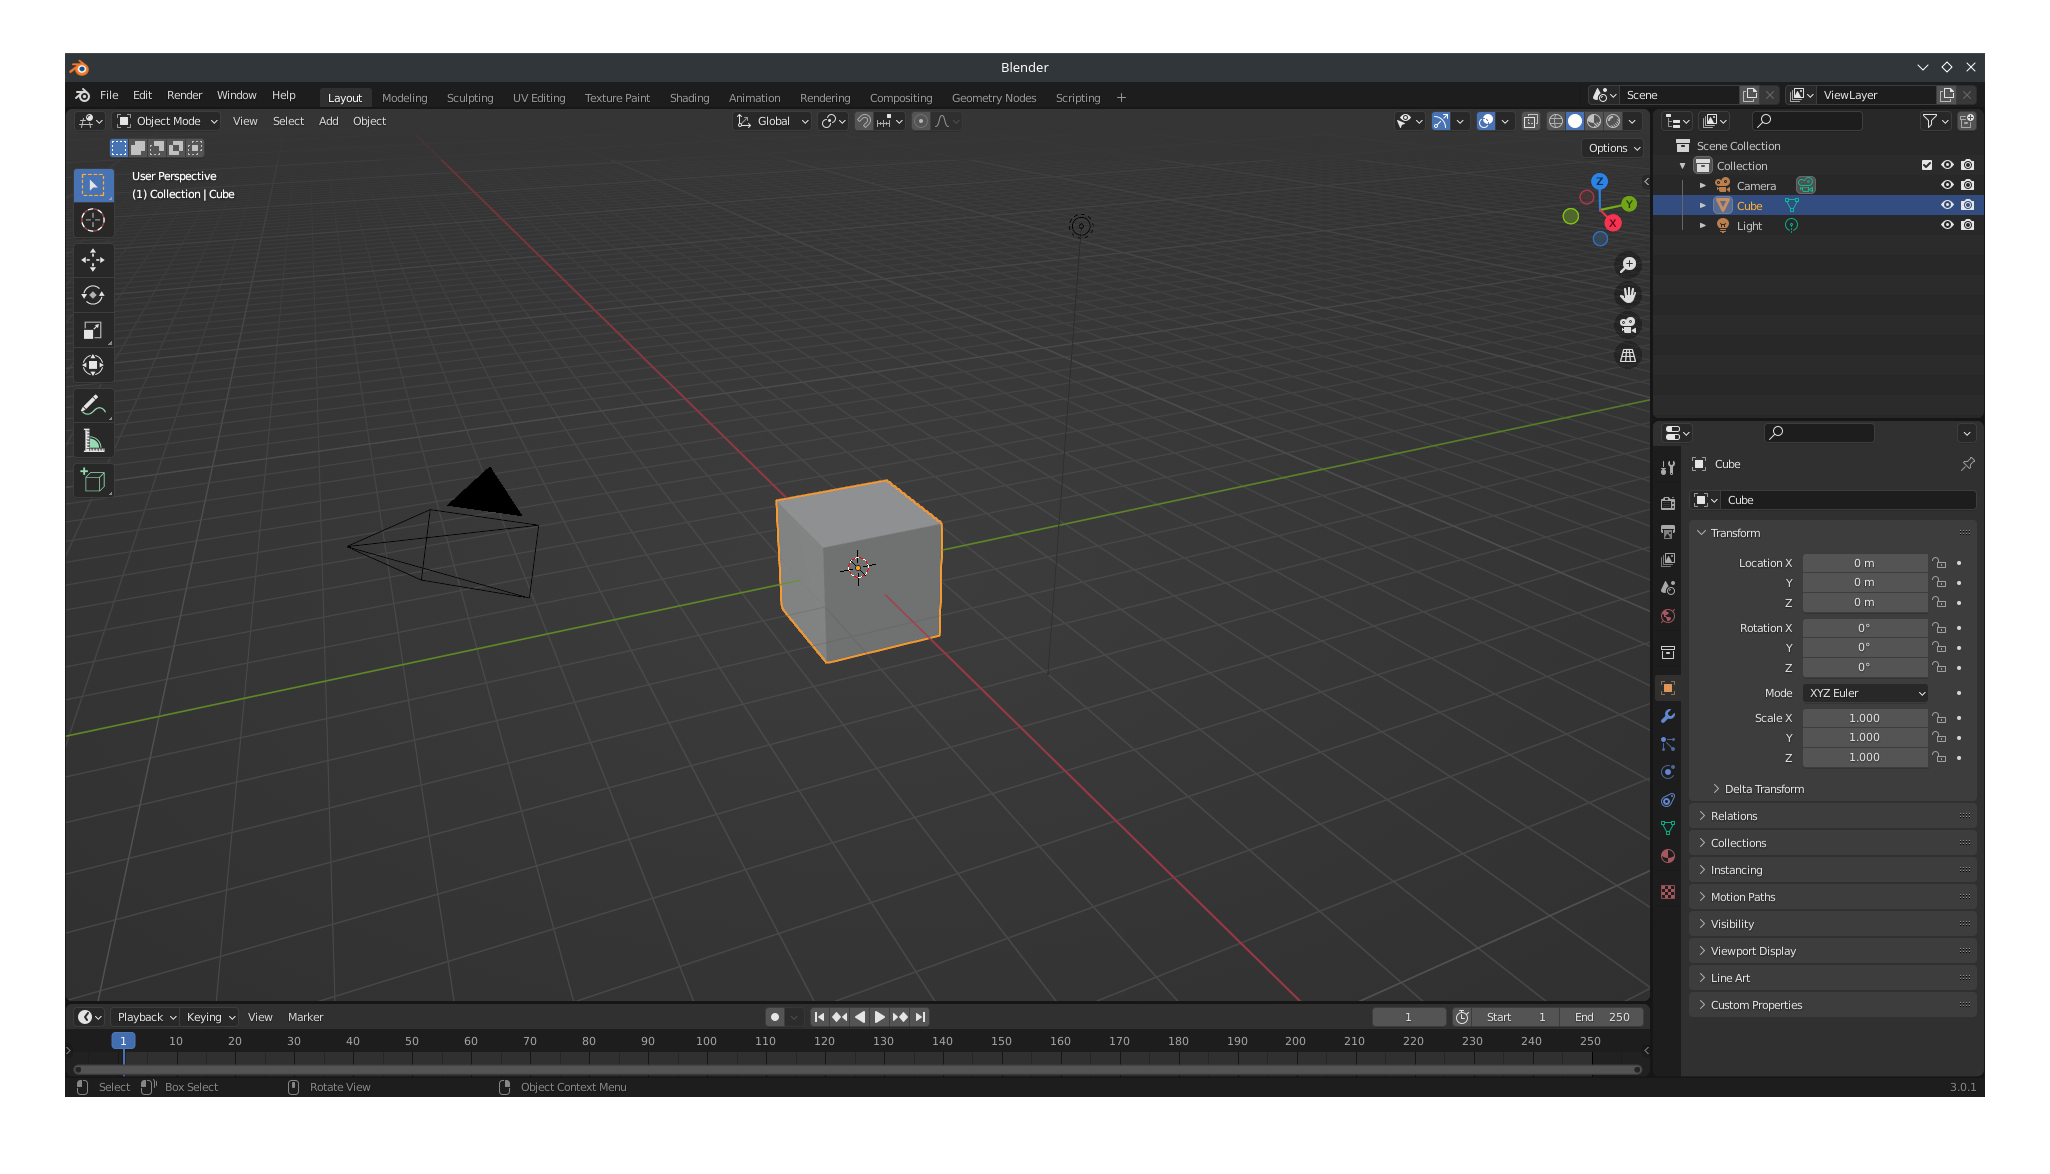
\includegraphics[width=0.9\textwidth]{images/blender.png}
	\caption{Interfejs programu Blender \cite{BLENDER} używanego do modelowania 3D}
	\label{blendermodel}
\end{figure}


\subsubsection{Formaty opisu sceny glTF}

Liczba możliwych elementów składającymi się na zasób 3D skłoniła branżę do opracowania ustandaryzowanych formatów opisu sceny, wśród których szczególną popularność zdobyły:
\begin{itemize}
	\item \textit{FBX} (Filmbox): rozwijany od 2006 przez Autodesk zamknięty format szeroko używany w branży gier z powodu łatwego eksportu oferowanego przez programy Autodesk 3ds Max i Maya.
	Jego zamknięta natura wymaga importowania albo przy pomocy oficjalnego SDK wymagającego akceptacji restrykcyjnego EULA, albo reimplementacji wymaganych części formatu inżynierią wsteczną.
	\item \textit{USD} (Universal Scene Description): otwarty format rozwijany od 2016 przez Pixar pozwala na łatwą i kompletną wymianę informacji pomiędzy różnymi najnowocześniejszymi programami grafiki 3D używanymi przez Pixar do produkcji animacji.
	Jego skompresowany i okrojony zamknięty wariant \textit{USDZ} jest używany przez Apple.
	\item \textit{glTF} (Graphics Language Transmission Format): rozwijany od 2015 przez Khronos otwarty format przystosowany do przechowywania ostatecznej wersji sceny w sposób prosty do sparsowania i wyrenderowania bądź dalszego przetworzenia.
	Wersja 2.0 wydana w 2021 zerwała kompatybilność wsteczną z wersją 1.0 i całkowicie ją zastąpiła.
\end{itemize}

Wśród wymienionych formatów jedynie glTF jest w pełni otwarty i łatwo importowany, dlatego jest on dobrym wyborem jako format zasobów 3D używanych przez silnik graficzny. Na przykład Godot \cite{godotengine} wspiera glTF jako główny i rekomendowany format opisy sceny.

Zgodnie ze specyfikacją glTF \cite{GLTFSPEC} zasób jest reprezentowany przez:
\begin{itemize}
	\item plik tekstowy \textit{*.gltf} w formacie JSON zawierający pełny opis sceny i jej poszczególnych elementów,
	\item pliki binarne \textit{*.bin} zawierający dane buforów zawierających geometrię bądź animacje,
	\item pliki obrazów \textit{*.png} i \textit{*.jpg} opisujące tekstury,
\end{itemize}
Pliki binarne i obrazy mogą być osadzone bezpośrednio w obiecie JSON używając kodowania Base64.
Możliwe jest też użycie binarnej wersji formatu glTF pozwalający na przechowywanie wszystkich danych w jednym binarnym pliku \textit{.glb}.

Zasób glTF składa się z obiektu JSON zawierającego metadane oraz osobne tablice dla każdego typu elementu zasobu.
Elementy mogą odnosić się do innych elementów używając ich indeksów w odpowiednich tablicach.
Relacje pomiędzy różnymi typami elementów zostały pokazana na poniższym diagramie:
\begin{figure}[H]
	\centering
	\begin{tikzpicture}[node distance=0.5cm]
		\tikzstyle{entity} = [rectangle, minimum width=2cm, minimum height=0.5cm,text centered, draw=black]
		\tikzstyle{refers} = [thick,->,>=stealth]
		
		\node (scene) [entity] {scene};
		\node (node) [entity, below = of scene] {node};
		\node (mesh) [entity, below = of node] {mesh};
		\node (accessor) [entity, below = of mesh] {accessor};
		\node (bufferView) [entity, below = of accessor] {bufferView};
		\node (buffer) [entity, below = of bufferView] {buffer};
		
		\node (camera) [entity, above right = of node] {camera};
		\node (skin) [entity, left = of node] {skin};
		\node (animation) [entity, below = of skin] {animation};
		
		\node (material) [entity, right = of accessor] {material};
		\node (texture) [entity, below = of material] {texture};
		\node (image) [entity, below = of texture] {image};
		\node (sampler) [entity, right = of image] {sampler};
		
		\draw [refers] (scene) edge[] (node);
		\draw [refers] (node) edge[] (mesh);
		\draw [refers] (mesh) edge[] (accessor);
		\draw [refers] (accessor) edge[] (bufferView);
		\draw [refers] (bufferView) edge[] (buffer);
		\draw [refers] (node) edge[out=-5,in=5, loop] (node);
		\draw [refers] (node) edge[] (camera);
		\draw [refers] (mesh) edge[] (material);
		\draw [refers] (material) edge[] (texture);
		\draw [refers] (texture) edge[] (image);
		\draw [refers] (texture) edge[] (sampler);
		\draw [refers] (node) edge[] (skin);
		\draw [refers] (skin) edge[] (node);
		\draw [refers] (skin) edge[out=-10,in=180,looseness=0] (accessor);
		\draw [refers] (animation) edge[] (node);
		\draw [refers] (animation) edge[] (accessor);
		
	\end{tikzpicture}
	\caption{Relacje pomiędzy rożnymi typami elementów w formacie glTF}
	\label{gltf_concepts}
\end{figure}

// TODO Opisz poszczególne typy elementów?

Przykładowo plik \textit{triangle.gltf} opisujący scenę zawierającą pojedyńczy trójkątą z geometrią składającą się z wierzchołków pozycji zawartych w pliku \textit{triangle.bin} wygląda następująco:

\noindent\begin{minipage}{.35\textwidth}
\lstset{language=JSON}
\begin{lstlisting}
{
  "asset" : {
    "version" : "2.0"
  },
  "scene" : 0,
  
  "scenes" : [
  {
    "nodes" : [ 0 ]
  } ],
  "nodes" : [
  {
    "mesh" : 0
  } ],
  "meshes" : [
  {
    "primitives" : [ {
      "attributes" : {
        "POSITION" : 0
      }
    } ]
  } ],
\end{lstlisting}
\end{minipage}\hfill
\begin{minipage}{.55\textwidth}
\lstset{language=JSON}
\begin{lstlisting}[frame=l]
  "buffers" : [
  {
    "uri" : "triangle.bin",
    "byteLength" : 36
  } ],
  "bufferViews" : [
  {
    "buffer" : 0,
    "byteOffset" : 0,
    "byteLength" : 36,
    "target" : 34962
  } ],
  "accessors" : [
  {
    "bufferView" : 0,
    "byteOffset" : 0,
    "componentType" : 5126,
    "count" : 3,
    "type" : "VEC3",
    "max" : [ 1.0, 1.0, 0.0 ],
    "min" : [ 0.0, 0.0, 0.0 ]
  } ]
}
\end{lstlisting}
\end{minipage}

\subsection{Zasoby wyjściowe}

Zasoby wyjściowe mają formę plików w formacie przystosowanym do manipulacji przez aplikację. Przykładami zasobów wyjściowych są pliki z rozszerzeniami \textit{.uasset} i \textit{.umap} używane przez silnik Unreal Engine \cite{unrealengine} do przechowywania zasobów w zoptymalizowanym formacie binarnym czy pliki \textit{.streamdb} i \textit{.resources}, które według twórców narzędzia do ekstrakcji zasobów z gier UnArch \cite{UNARCH} są używane w grze Doom Eternal i zastąpiły pliki \textit{.pak} wcześniejszych gier od id Software.


\subsection{Potok zasobów}

Potok zasobów (ang. asset pipeline) to część silnika odpowiadająca za konwersję zasobów wejściowych na zasoby wyjściowe.
Konwersja ta jest wymagana, ponieważ istnieją różne wymagania dotyczące formatów: zasoby wejściowe są zoptymalizowane pod kątem oszczędności miejsca na dysku i interoperacyjności między oprogramowaniem zewnętrznym, kiedy zasoby wyjściowe zwykle wymagają mniejszego zakresu możliwych funkcjonalności i powinny być w formacie dostosowanym do maksymalnie szybkiego wczytywania przez aplikację - szybkość ich zapisu jest mniej ważna ponieważ musi się odbyć tylko jeden raz na komputerach twórców oprogramowania uruchamiających potok zasobów.

\subsection{Baza zasobów}
Baza zasobów (ang. asset database) to zasób wyjściowy mający na celu zgromadzenie informacji o wszystkich zasobach używanych przez silnik.
// HIRO



// TODO

\section{Graf sceny}

// TODO hierarchical modeling

\section{Graf renderowania}

// TODO